\documentclass[12pt,a4paper,twoside,openright]{book}

\setlength{\oddsidemargin} {2. cm}
\setlength{\evensidemargin} {2. cm}
\addtolength{\oddsidemargin} {-0.4 cm}
\addtolength{\evensidemargin} {-0.4 cm}
\linespread{1.1}

\usepackage[italian]{babel}
\usepackage[latin1]{inputenc}
\usepackage{amsmath}

% La descrizione di figure e tabelle
\usepackage{graphicx}\usepackage[margin=20pt, font=small, labelfont=bf]{caption}

\usepackage{hyperref}		% Link interni clickabili

% Informazioni che vengono inserite come descrizione del PDF prodotto.
\hypersetup{
	pdftitle = {Cinetica chimica},
	pdfsubject = {Appunti del corso tenuto da C. Cavallortti al Politecnico di Milano},
	pdfkeywords = {cinetica, chimica, appunti, polimi},
	pdfauthor = {\textcopyright\ Marco Vito Moscaritolo},
	pdfcreator = {\LaTeX},
	pdfproducer = {pdfeTeX-0.\the\pdftexversion\pdftexrevision},
}

% Imposta il colore dei link.
\hypersetup{colorlinks=true,
						linkcolor=magenta,		% Colore dei link interni al documento
						anchorcolor=magenta,	% Colore dei link ad ancore
						citecolor=magenta,		% Colore dei link a fonti bibliografiche
						filecolor=magenta,		% Colore dei link a file locali
						menucolor=magenta,		% Colore dei link nel menu di adobe Acrobat Reader
						pagecolor=magenta,		% Colore dei link ad altre pagine
						urlcolor=magenta,			% Colore dei link a url
					 }
					 
\begin{document}

	\thispagestyle{empty}

\vspace*{-1.5cm} 

\begin{center}
  \large
  POLITECNICO DI MILANO\\
  \normalsize
  Corso di Laurea in Ingegneria Chimica\\
  Dipartimento di Chimica e de Materiali "Natta"
  
  \vspace*{3cm} 
  
  \LARGE
  \textbf{Cinetica chimica applicata}
  
  \vspace*{1.5cm}

  \normalsize
  Prof: Carlo Cavallotti
\end{center}
\vspace*{6.0cm}
\begin{flushright}


  Appunti di:\\ 
  	Marco Vito Moscaritolo\\ 
	\href{mailto:mavimo@gmail.com}{mavimo@gmail.com}\\
	\href{http://mavimo.netsons.org}{Web site}

\end{flushright}
\vspace*{0.5cm}
\begin{center}
	Anno Accademico 2005-2006
\end{center}
\clearpage

\begin{figure*}
	\centering
		
\includegraphics{image/CCsomerights.pdf}
	\label{fig:CCsomerights}
\end{figure*}

\small
\noindent Il contenuto di questo documento � distribuito secondo la:
\begin{center}
	\Large
	\textbf{Creative Commons Licence v 2.5}\\
	\small Attribuzione - Non commerciale - Non opere derivate
\end{center}

\vspace{1cm}

\noindent Potete trovare il testo completo della licenza al seguente link:\\
\begin{center}
\url{http://creativecommons.org/licenses/by-nc-nd/2.5/it/}
\end{center}

\vspace{5cm}

\normalsize
\noindent Versioni precedenti:

\small
\begin{itemize}
	\item 1.2.5 - 11/09/2006 - Correzioni al Capitolo 5
	\item 1.2.4 - 11/09/2006 - Correzioni al Capitolo 4
	\item 1.2.3 - 10/09/2006 - Correzioni al Capitolo 3
	\item 1.2.2 - 05/09/2006 - Correzioni al Capitolo 2
	\item 1.2.1 - 01/09/2006 - Correzioni al Capitolo 1
	\item 1.1 - 20/07/2006 - Inserita Appendice A
	\item 1.0 - 01/07/2006 - Termine prima stesura del documento
\end{itemize}

 




	
	\frontmatter
		\tableofcontents
	\clearpage

  \mainmatter
		\chapter{Isoterme}
%===============================================================================================
\section{Isoterma B.E.T.}
L'isoterma B.E.T (sviluppata da 
Brauneuer\footnote{Dire chi �...}, 
Emmett\footnote{Emmett, Paul Hugh (Portland 1900 - 1985), Chimico americano } e 
Teller\footnote{Teller, Edward (Ungheria 1908 - America 2003), Fisico nucleare}) 
si basa su di un approccio di tipo statistico, in cui una superficie che espone dei punti di adsorbimento (siti) viene coperta da uno o pi� strati di molecole di gas, come � visibile in \figurename~\ref{fig:BET:SchemaMolecole}

\begin{figure}[htbp]
	\centering
		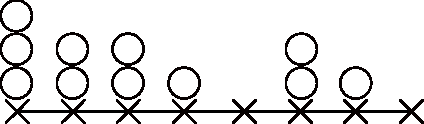
\includegraphics[width=0.50\textwidth]{image/BETSchemaMolecole.pdf}
	\caption{Schema rappresentativo della teoria alla base dell'\textit{isoterma B.E.T.}}
	\label{fig:BET:SchemaMolecole}
\end{figure}

Utilizzeremo $\vartheta_i$ per indicare la frazione dei siti ricoperti da $i$ strati di molecole, quindi sar� anche verificato:
\begin{equation}
	\vartheta_0 + \sum^\infty_{i=1}\vartheta_i = 1
	\label{eq:SommaEpsilon}
\end{equation}

Il simbolo $\sigma$ rappresenta il numero di molecole adsorbite per unit� di area e pu� essere determinato come:
\begin{equation}
	\sigma = \sum^n_{i=1}\vartheta_i \cdot \sigma_m \cdot i
	\label{eq:Sigma}
\end{equation}
dove $\sigma_m$ indica il numero di siti per unit� di area presenti sulla superficie.

Consideriamo ora le reazioni di adsorbimento dei vari strati:
\begin{align}
	G + S_0 \underset{r_{des^1}}{\overset{r_{ad^1}}{\rightleftharpoons}} S_1 \\
	G + S_1 \underset{r_{des^2}}{\overset{r_{ad^2}}{\rightleftharpoons}} S_2 \\
	\dots  \\
	G + S_{n-1} \underset{r_{des^n}}{\overset{r_{ad^n}}{\rightleftharpoons}} S_n
	\label{reaz:Adsorbimento}
\end{align}
essendo per definizione
\begin{align}
	r_{ads}^i = K_{ads}^i \cdot G \cdot \vartheta_{1-i} \cdot \sigma_m	\\
	r_{des}^i = K_{des}^i \cdot \vartheta_{i} \cdot \sigma_m
	\label{eq:VelAdDes}
\end{align}
Che scritte per la serie di reazioni prima considerate porta ad avere,
considerando di essere all'equalibrio ($r_{ads}^i = r_{des}^i$), ed 
essendo la concentrazione del gas $G = \frac{n}{V}=\frac{P}{R T}$:
\begin{align}
	K_{ads}^{1} \cdot \frac{P}{R T} \cdot \vartheta_{0} \cdot \sigma_m	& =  K_{des}^{1} \cdot \vartheta_{1} \cdot \sigma_m \\
	K_{ads}^{2} \cdot \frac{P}{R T} \cdot \vartheta_{1} \cdot \sigma_m	& =  K_{des}^{2} \cdot \vartheta_{3} \cdot \sigma_m \\
	\dots \\
	K_{ads}^{\infty} \cdot \frac{P^0}{R T} \cdot \sigma_m	& =  K_{des}^{\infty} \cdot \sigma_m
	\label{eq:EquilAdsDes}
\end{align}
L'ultima equazione � ottenuta dal fatto che, quando sulla superficie vi � un film di liquido, 
la pressione � pari alla tensione di vapore e i gradi di ricoprimento possono essere ritenuti 
unitari.

Le costanti di adsorbimento possono essere ritenute costanti, inquanto ci si trova a T basse 
(liquefazione di gas), quindi l'energia cinetica delle molecole � bassa e tutte le particelle 
gassose che raggiungono la superficie vi aderiscono. \\
Le costanti di desorbimento, invece, possono essere ritenute costanti solo per gli strati superiori
perch� non risentono delle interazioni con gli atomi vicini, quindi:
\begin{align}
	K_{ads}^{1} = K_{ads}^{2} = K_{ads}^{3} = \dots = K_{ads}^{n} = K_{ads}\\
	K_{des}^{1} \neq K_{des}^{2} = K_{des}^{3} = \dots = K_{des}^{n} =K_{des}
	\label{eq:CostEqAdsDes}
\end{align}

Dividiamo ora le costanti di equilibrio del primo e dell'$i$-esimo strato per le equazioni di 
equilibrio dello strato $\infty$ (equazioni \ref{eq:EquilAdsDes}) ottenendo:
\begin{align}
	\frac{K_{ads} \cdot \frac{P}{R T} \cdot \vartheta_{0} \cdot \sigma_m}{K_{ads} \cdot \frac{P^0}{R T} \cdot \sigma_m} = &
	\frac{K_{des}^{1} \cdot \vartheta_{1} \cdot \sigma_m}{K_{des} \cdot \sigma_m} & \Longrightarrow &
	\frac{P}{P^0} \cdot \vartheta_0 = \frac{K_{des}^1}{K_{des}} \cdot \vartheta_1 \\
	\frac{K_{ads} \cdot \frac{P}{R T} \cdot \vartheta_{i-1}}{K_{ads} \cdot \frac{P^0}{R T}} = &
	\frac{K_{des} \cdot \vartheta_{i} \cdot \sigma_m}{K_{des} \cdot \sigma_m} & \Longrightarrow &
	\frac{P}{P^0} \cdot \vartheta_{i-1} = \vartheta_{i}
	\label{eq:RappEqui}
\end{align}

Sostituendo il valore di $\vartheta_{i-1}$ con quello di ricavato da $\vartheta_{i-2}$ e
 proseguendo cos� fino a $1$ otterremmo:
\begin{align}
	\vartheta_i = \left( \frac{P}{P^0}\right)^{i-1} \cdot \vartheta_1 = x^{i-1} \cdot \vartheta_1
	\label{eq:EpsilonI}
\end{align}
avendo sostituito $x = \frac{P}{P^0}$. 
Ricavando il valore di $\vartheta_1$ dall'equilibrio (equazione \ref{eq:EquilAdsDes}) 
\begin{align}
	\vartheta_1 = \frac{K_{ads}}{K_{des}^1} \frac{P}{R T} \vartheta_0 
	\label{eq:Epsilon1Equil}
\end{align}
Che sostituita nell'equazione \ref{eq:EpsilonI} porta a:
\begin{align}
	\vartheta_i = \left( \frac{P}{P^0}\right)^{i-1} \cdot \frac{K_{ads}}{K_{des}^1} \frac{P}{R T} \vartheta_0
	\label{eq:EpsilonIEqu}
\end{align}
Moltiplicando e dividendo per $P^0$ e ricordando il significato di $x$ otteniamo:
\begin{align}
	\vartheta_i = \left( \frac{P}{P^0}\right)^{i-1} \cdot \frac{K_{ads}}{K_{des}^1} 
							\frac{P}{R T} \vartheta_0 \cdot \frac{P^0}{P^0} =
							\frac{K_{ads}}{K_{des}^1} \frac{P^0}{R T} x^i \cdot \vartheta_0 =
							C \cdot x^i \cdot \vartheta_0
	\label{eq:EpsilonIFin}
\end{align}
Avendo accorpato in una costante i termini fissi, ovvero $C = \frac{K_{ads}}{K_{des}^1} \frac{P^0}{R T}$

Sostituendo il risultato ottenuto (equazione \ref{eq:EpsilonIFin}) nelle equazioni \ref{eq:SommaEpsilon} e \ref{eq:Sigma} otteniamo:
\begin{equation}
	\vartheta_0 + \sum^\infty_{i=1}\left(C \cdot x^i \cdot \vartheta_0\right) = 1
	\label{eq:SommaEpsilonSost}
\end{equation}
e
\begin{equation}
	\sigma = \sum^n_{i=1}\left(C \cdot x^i \cdot \vartheta_0 \cdot \sigma_m \cdot i\right)
	\label{eq:SigmaSost}
\end{equation}

Il rapporto tra i due termini diventer�:
\begin{equation}
	\frac{\sigma}{1} = 
	\frac	{\sum^n_{i=1}\left(C \cdot x^i \cdot \vartheta_0 \cdot \sigma_m \cdot i\right)}
				{\vartheta_0 + \sum^\infty_{i=1}\left(C \cdot x^i \cdot \vartheta_0\right)}
	\label{eq:RapSigmaUpsilon}
\end{equation}

Le due sommatorie convergono per $\left|x\right| < 1$, infatti:
\begin{equation}
	\sum^{\infty}_{i=1} i \cdot x^i = \frac{x}{(1-x)^2}
	\label{eq:ConvSum1}
\end{equation}
\begin{equation}
	\sum^{\infty}_{i=1} x^i = \sum^{\infty}_{i=1} x^i - 1 = \frac{x}{1-x}
	\label{eq:ConvSum2}
\end{equation}

Note queste caratteristiche delle sommatorie, e tornando all'equazione \ref{eq:RapSigmaUpsilon} otteniamo:
\begin{equation}
	\sigma = 
	\frac	{C \cdot \vartheta_0 \cdot \sigma_m  \frac{x}{(1-x)^2}}
				{\vartheta_0 + \vartheta_0 \cdot C \cdot \frac{x}{1-x}} =
				\frac	{C \cdot \sigma_m  \frac{x}{(1-x)^2}}
							{1 + C \cdot \frac{x}{1-x}} 
	\label{eq:RapSigmaUpsilonSum}
\end{equation}
Che riarrangiando permettono di ottenere:
\begin{equation*}
	\left[ 1 + C \cdot \frac{x}{1-x} \right] \frac{1}{C \cdot \sigma_m} = 
	\frac{1}{\sigma} \cdot \frac{x}{(1-x)^2}
\end{equation*}
\begin{equation*}
	\left[ 1 + C \cdot \frac{x}{1-x} \right] \frac{1}{C \cdot \sigma_m} \cdot (1-x) = 
	\frac{1}{\sigma} \cdot \frac{x}{(1-x)}
\end{equation*}
\begin{equation*}
	\left[ 1 - x + C \cdot x \right] \frac{1}{C \cdot \sigma_m} = 
	\frac{1}{\sigma} \cdot \frac{x}{(1-x)}
\end{equation*}
\begin{equation}
	\frac{1}{C \cdot \sigma_m} + x \cdot \frac{C - 1}{C \cdot \sigma_m} = 
	\frac{1}{\sigma} \cdot \frac{x}{(1-x)}
	\label{eq:RapSigmaUpsilonSumRiarr}
\end{equation}
Ricordando il significato di $x$ e sapendo che $\frac{\sigma}{\sigma_m} = \frac{V_{ads}}{V_m}$
dall'equazione precedente otteniamo:
\begin{equation}
	\frac{1}{C \cdot \sigma_m} + \frac{P}{P^0} \cdot \frac{C - 1}{C \cdot \sigma_m} =
	\frac{P}{P^0} \cdot \frac{\frac{P}{P^0}}{1-\frac{P}{P^0}} \cdot \frac{1}{\sigma_m \cdot \frac{V_{ads}}{V_m}} =
	\frac{1}{C \cdot \sigma_m} + \frac{P}{P^0} \cdot \frac{C -1}{C \cdot \sigma_m}
	\label{eq:RapSigmaUpsilonSumRiarrFin}
\end{equation}
che linearizzata ci permette di ottenere:
\begin{equation}
	\frac{P}{P-P^0} - \frac{1}{V_{ads}} = 
	\frac{1}{C \cdot V_{ads}} + \frac{P^0}{P} \cdot \frac{C - 1}{C \cdot V_m}
	\label{eq:BETLinearizzata}
\end{equation}
Tramite prove sperimentali � possibile ricavare $C$ e $V_m$ e di conseguenza l'equazione � completata e permette di correlare il volume adsorbito ($V_{ads}$) con la pressione del gas ($P$).
%================================================================================================
\section{Isoterma di Langmuir}
Indichiamo con $^*$ la specie adsorbita, e ricordando l'equazione \ref{eq:SommaEpsilon}, introduciamo la variabile $\Gamma^0$ che rappresenta la concentrazione totale dei siti superficiali, � quindi evidente che:
\begin{equation}
	C_i^{*} = \vartheta_i^{*} \cdot \Gamma^0
	\label{eq:ConcStar}
\end{equation}
\begin{equation}
	\sigma = \vartheta_i \cdot \Gamma^0
	\label{eq:ConcSpecie}
\end{equation}
dove $C^{*}$ indica la concentrazione della specie $i$-esima adsorbita e con $\sigma$ la concentrazione dei siti liberi.
Sar� dunque vero anche:
\begin{equation}
	\sigma + \sum_{i=1}^{NS} C_i^{*} = \Gamma^0
	\label{eq:ValGamma0}
\end{equation}
dove $NS$ � il numero di specie che possono essere adsorbite.

Dividendo ambo i membri dell'equazione precedente per $\Gamma^0$ � evidente che:
\begin{equation}
	\frac{\sum_{i=1}^{NS}C_i^{*}}{\Gamma^0} + \frac{\sigma}{\Gamma^0} = \frac{\Gamma^0}{\Gamma^0} =1
	\label{eq:GammaSuGamma}
\end{equation}
e per le equazioni \ref{eq:ConcStar} e \ref{eq:ConcSpecie} anche:
\begin{equation}
	\sum_{i=1}^{NS} \vartheta_i^{*} + \vartheta_i = 1
	\label{eq:SommaUpsilon}
\end{equation}

Scrivendo la generica reazione di adsorbimento e desorbimento abbiamo:
\begin{equation}
	A + \sigma \stackrel{K_{ads}}{\rightarrow} A^{*}
	\label{eq:RxnAds}
\end{equation}
\begin{equation}
	A^{*} \stackrel{K_{des}}{\rightarrow} A + \sigma
	\label{eq:RxnAds2}
\end{equation}
le cui velocit� risulteranno, rispettivamente:
\begin{equation}
	r_{ads} = K_{ads} \cdot C_{A} \cdot C_{\sigma} 
	\label{eq:VelRxnAds}
\end{equation}
\begin{equation}
	r_{des} = K_{des} \cdot C_{A^{*}} 
	\label{eq:VelRxnAds2}
\end{equation}

Applicando il P.S.S.A. sulle specie superficiali abbiamo:
\begin{equation}
	\frac{\partial C_{A^{*}}}{\partial t} = 0
	\label{eq:PSSAAStar}
\end{equation}
\begin{equation}
	\frac{\partial C_{\sigma}}{\partial t} = 0
	\label{eq:PSSACSigma}
\end{equation}
ma anche, considerando una sola specie che si adsorbe:
\begin{equation}
	C_{A^{*}} + C_{\sigma} = \Gamma^0
	\label{eq:SitiOccupati}
\end{equation}
come conseguenza dell'equazione \ref{eq:PSSAAStar} si ha $r_{ads} = r_{des}$ ed esplicitandole:
\begin{equation}
	\left\{
		\begin{array}{l}
			K_{ads} \cdot C_A \cdot C_{\sigma} = K_{des} \cdot C_{A^{*}} \\
			C_{A^{*}} + C_{\sigma} = \Gamma^0
		\end{array}
	\right.
	\label{eq:VelRxnEquil}
\end{equation}
Ricavando $C_{A^{*}}$ dal sistema di equazioni \ref{eq:VelRxnEquil} abbiamo:
\begin{equation}
	C_{A^{*}} = \Gamma^0 - C_{\sigma} = \frac{K_{ads}}{K_{des}} \cdot C_A \cdot C_{\sigma}
	\label{eq:VelRxnEquilSost}
\end{equation}
da cui, isolando $C_{\sigma}$, otteniamo:
\begin{equation}
	C_{\sigma} = \frac{\Gamma^0}{1 + \frac{K_{ads}}{K_{des}} \cdot C_A}
	\label{eq:CSigma}
\end{equation}
e per la definizione di $C_{A^{*}}$ dell'equazione \ref{eq:VelRxnEquilSost} abbiamo:
\begin{equation}
	C_{A^{*}} = \frac{K_{ads}}{K_{des}} \cdot C_A \cdot C_{\sigma} = 
	\frac{\Gamma^0 \cdot \frac{K_{ads}}{K_{des}} \cdot C_A}
				{1 + \frac{K_{ads}}{K_{des}} \cdot C_A} = 
	\frac{\Gamma^0 \cdot K_{eq}^{ads} \cdot C_A}
				{1 + {K_{eq}^{ads} \cdot C_A}}
	\label{eq:CAStar}
\end{equation}
dove $K_{eq}^{ads}$ � la costante di equilibrio del processo di adsorbimento/desorbimento. Nel medesimo modo � possibile ricavare $\vartheta_{A^{*}}$ essendo, per l'equazione \ref{eq:ConcStar}:
\begin{equation}
	\vartheta_{A^{*}} = \frac{C_{A^{*}}}{\Gamma^0} =
	\frac{K_{eq}^{ads} \cdot C_A}
				{1 + K_{eq}^{ads} \cdot C_A}
	\label{eq:UpsilonAStar}
\end{equation}

Se pi� specie possono adsorbirsi � possibile applicare lo stesso procedimento a condizione di inserire nel sistema iniziale $N-1$ equazioni delle specie adsorbite a cui � applicato il P.S.S.A. e ricordarsi che:
\begin{equation}
	\Gamma^0 = \sum C_{i^{*}} + C_{\sigma}
	\label{eq:GammaSomma}
\end{equation}
il sistema iniziale, utilizzando una serie di reazioni, sarebbe:
\begin{equation}
	\left\{
		\begin{array}{l}
			K^{ads}_{A} \cdot C_A \cdot C_{\sigma} = K^{des}_{A} \cdot C_{A^{*}}\\
			K^{ads}_{B} \cdot C_B \cdot C_{\sigma} = K^{des}_{B} \cdot C_{B^{*}}\\
			K^{ads}_{C} \cdot C_C \cdot C_{\sigma} = K^{des}_{C} \cdot C_{C^{*}}\\
			\dots \\
			\sum_{j=1}^{NC} C_j + C_{\sigma} = \Gamma^0
		\end{array}
	\right.
	\label{eq:RxnMulticomp}
\end{equation}
il cui risultato sarebbe:
\begin{equation}
	C_{\sigma} = \frac{\Gamma^0}{1 + \sum_{j=1}^{NC}K_{eq_j}^{ads} \cdot C_j}
	\label{eq:CSigmaFinale}
\end{equation}
\begin{equation}
	C_{i^{*}} = 
	\frac{\Gamma^0 \cdot K_{eq_i}^{ads} \cdot C_i}
				{1 + \sum_{j=1}^{NC}{K_{eq_j}^{ads} \cdot C_j}}
	\label{eq:CIStarMulti}
\end{equation}

%================================================================================================
\section{Meccanismo LHHW}
Il meccanismo LHHW (Langmuir\footnote{Langmuir, Irving (New York 1881 - Falmouth, Massachusetts 1957), chimico statunitense.}-Hinshelwood\footnote{Hinshelwood, Cyril Norman (Londra 1897-1967), chimico britannico.}) si basa sulla teoria di Langmuir e considera la reazione tra le due specie reattive solo se sono adsorbite sulla superficie, quindi il meccanismo complessivo pu� essere suddiviso in
\begin{enumerate}
	\item Trasporto dei reagenti dal bulk all'interfaccia
	\item	Adsorbimento dei reagenti
	\item Reazione superficiale
	\item	Desorbimento dei prodotti
	\item	Diffusione dei prodotti dall'interfaccia al bulk
\end{enumerate}

Trascurando i fenomeni di trasporto, per una reazione del tipo:
\begin{equation}
	A \rightarrow B
	\label{eq:LHHW_Rxn_tot}
\end{equation}
Possiamo rappresentare i punti 2, 3 e 4 come:
\begin{equation}
	\begin{array}{l}
		A + \sigma \rightarrow A^{*} \\
		A^{*} \rightarrow B^{*} \\
		B^{*} \rightarrow B + \sigma \\
	\end{array}
	\label{eq:LHHW_Rxn}
\end{equation}

Supponendo un R.D.S.\footnote{Rate Determining Step} per la seconda reazione abbiamo:
\begin{equation}
	\begin{array}{rl}
				r_1 & = \overset{\rightarrow}{k_1} \cdot C_{A} \cdot C_{\sigma} 
					- \overset{\leftarrow}{k_1} \cdot C_{A^{*}} \\
		R = r_2 & = \overset{\rightarrow}{k_2} \cdot C_{A^{*}} 
					- \overset{\leftarrow}{k_2} \cdot C_{B^{*}} \\
				r_1 & = \overset{\rightarrow}{k_3} \cdot C_{B^{*}}  
					- \overset{\leftarrow}{k_3} \cdot C_{B} \cdot C_{\sigma}
	\end{array}
	\label{eq:LHHW_r}
\end{equation}

Essendo all'equilibrio $r_1=r_3=0$ (siamo all'equilibrio per queste due reazioni), quindi:
\begin{equation}
	\begin{array}{cp{2cm}c}
				K_{eq}^1 = \frac{C_{A^{*}}}{C_A \cdot C_{\sigma}}	&
				 &
				K_{eq}^3 = \frac{C_B \cdot C_{\sigma}}{C_{B^{*}}}	
	\end{array}
	\label{eq:LHHW_keq}
\end{equation}
Ricordando anche che:
\begin{equation}
	\Gamma^0 = C_{\sigma} + C_{B^{*}} + C_{A^{*}}
	\label{eq:LHHW_Gamma0}
\end{equation}
Se ricaviamo dalle costanti di equilibrio (equazioni \ref{eq:LHHW_keq}) $C_{A^{*}}$ e $C_{B^{*}}$, e le inseriamo nell'ultima equazione scritta (\ref{eq:LHHW_Gamma0}) ed esplicitandola rispetto a $C_{\sigma}$ otteniamo:
\begin{equation}
	C_{\sigma} = \frac{\Gamma^0}{1 + K_{eq^1} \cdot C_A + \frac{C_B}{K_{eq^3}}}
	\label{eq:LHHW_CSigma}
\end{equation}
Inserendo questa nelle equazioni di $C_{A^{*}}$ e $C_{B^{*}}$, ricavate dall'equazione \ref{eq:LHHW_keq}, otteniamo:
\begin{equation}
	C_{A^{*}} = \frac{K_{eq^1} \cdot C_A \cdot \Gamma^0}
	{1 + K_{eq^1} \cdot C_A + \frac{C_B}{K_{eq^3}}}
	\label{eq:LHHW_CAStar}
\end{equation}
\begin{equation}
	C_{B^{*}} = \frac{\frac{C_B}{K_{eq^3}} \cdot \Gamma^0}
									{1 + K_{eq^1} \cdot C_A + \frac{C_B}{K_{eq^3}}}
	\label{eq:LHHW_CBStar}
\end{equation}

Infine si ottiene, essendo $R = r_2$:
\begin{equation}
	R = r_2 = \overset{\rightarrow}{k_2} \cdot C_{A^{*}} - 	
						\overset{\leftarrow}{k_2} \cdot C_{B^{*}} = 
						\frac{\overset{\rightarrow}{k_2} \cdot \frac{C_B}{K_{eq^3}} - 
									\overset{\leftarrow}{k_2} \cdot K_{eq^1} \cdot C_A}
									{1 + K_{eq^1} \cdot C_A + \frac{C_B}{K_{eq^3}}} \cdot \Gamma^0
	\label{eq:LHHW_Rtot}
\end{equation}

Nel caso di reazioni del tipo
\begin{equation}
	A \rightarrow B + C
	\label{eq:LHHW_Rxn2}
\end{equation}

La reazione superficiale pu� avvenire in due modi differenti:
\begin{equation}
	A^{*} \rightarrow B^{*} + C
	\label{eq:LHHW_Rxn2modo1}
\end{equation}
oppure:
\begin{equation}
	A^{*} + \sigma \rightarrow B^{*} + C^{*}
	\label{eq:LHHW_Rxn2modo2}
\end{equation}

In base al meccanismo seguito la velocit� di reazione sar� differente, in particolare avremmo un meccanismo \textit{single-site} per la reazione \ref{eq:LHHW_Rxn2modo1} mentre \textit{dual-side} per la \ref{eq:LHHW_Rxn2modo2}. L'andamento risulter� simile a quanto rappresentato in \figurename~\ref{fig:LHHW:SingleDualSite}

\begin{figure}[htbp]
	\centering
		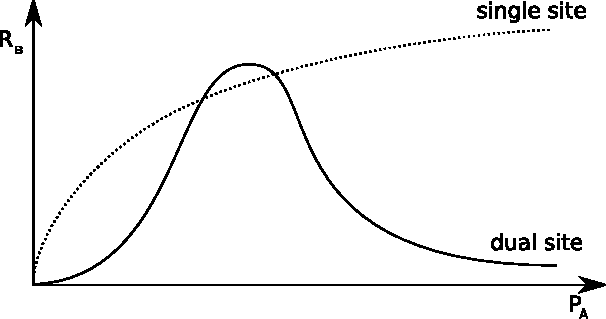
\includegraphics[width=0.50\textwidth]{image/LHHWSingleDualSite.pdf}
	\caption{Andamento della reazione secondo meccanismo \textit{single site} e \textit{dual site}.}
	\label{fig:LHHW:SingleDualSite}
\end{figure}







		\chapter{Teoria cinetica dei gas}
\section{Ipotesi}
La teoria cinetica dei gas si basa sulle seguenti ipotesi:
\begin{itemize}
	\item Elevata densit� molecolare
	\item	Elevata distanza intermolecolare rispetto le dimensioni delle molecole
	\item	Molecole non interagenti tra di loro
	\item	Distribuzione molecolare uniforme
	\item	Tutte le direzioni di moto equalmente probabili
\end{itemize}

\section{Energia cinetica del gas}
Consideriamo una superficie A contro cu avvengono gli urti delle molecole di gas, come raffigurato in \figurename~\ref{fig:TCG:UrtoParete}.
\begin{figure}[htbp]
	\centering
		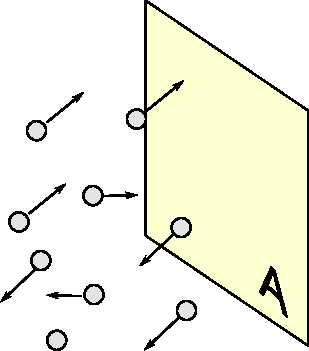
\includegraphics[width=0.40\textwidth]{image/TCGUrtoParete.pdf}
	\caption{Rappresenzatione schematica del meccanismo di base su cui si basa la Teoria Cinetica del Gas}
	\label{fig:TCG:UrtoParete}
\end{figure}
si possono determinare, per ogni particella, la distanza della parte:
\begin{equation}
	x = v_x \cdot \Delta t
	\label{eq:DistanzaParteParticella}
\end{equation}
e il numero di urti che subisce la partete:
\begin{equation}
	n_{urti} = \frac{1}{2} v_x \cdot \Delta t \cdot A \cdot N
	\label{eq:NumeroUrtiParete}
\end{equation}
dove $N$ � la densit� di molecole ($\frac{n}{V}$), mentre il fattore moltiplcativo $\frac{1}{2}$ � dovuto al fatto che le molecole si muovono nelle due direazioni di ogni asse, quindi solo la met� di esse avr� direzione utile per colpire la parte A.

La variazione di quantit� di moto a seguito di un urto � pari a:
\begin{equation}
	\Delta q = q_1 - q_2 = m \cdot v_x - (-v_x \cdot m) = 2 m \cdot v_x
	\label{eq:VariazQuantitaMoto1}
\end{equation}
dove la velocit� a seguito dell'urto ha direzione inversa, mentre, essendo l'urto elastico, ha lo stesso modulo.

La variazione della quantit� di moto totale sar� pari a:
\begin{equation}
	\Delta q_{TOT} = (\frac{1}{2} v_x \cdot \Delta t \cdot A \cdot N) \cdot (2 m \cdot v_x)
								 = m \cdot v_x^2 \cdot \Delta t \cdot A \cdot N
	\label{eq:VariazQuantitaMotoTot}
\end{equation}
che riarrangiata porta a 
\begin{equation}
	\frac{\Delta q_{TOT}}{A \cdot \Delta t} = m \cdot v_x^2 \cdot N
	\label{eq:VariazQuantitaMotoTotRiarr}
\end{equation}
Essendo $q = m \cdot v$, $a = \frac{v}{\Delta t}$, $F = m 	\cdot a$ e anche $P = \frac{F}{A}$ otteniamo:
\begin{equation}
	\frac{\Delta q_{TOT}}{A \cdot \Delta t} = \frac{F}{A} = P = m \cdot v_x^2 \cdot \frac{n}{V}
	\label{eq:Pressione}
\end{equation}
da cui ricaviamo anche:
\begin{equation}
	\frac{P V}{n} = m \cdot v_x^2
	\label{eq:EnergCientica1}
\end{equation}

Essendo per le ipotesi iniziali tutte le direzioni di moto egualmente probabili, si ha:
\begin{equation}
	<v>^2 = <v_x>^2 + <v_y>^2 + <v_z>^2 = 3 \cdot <v_x>^2
	\label{eq:Velocita2}
\end{equation}
quindi
\begin{equation}
	\frac{P V}{n} = R T =  m \cdot v_x^2 = m \cdot (\frac{1}{3} <v>^2)
	\label{eq:EnergCientica2}
\end{equation}
da cui si ricava il valore dell'energia cinetica media di un gas, che risulta essere paria a: 
\begin{equation}
	\frac{1}{2} m <v>^2 = \frac{3}{2} R \cdot T
	\label{eq:EnergCientica}
\end{equation}

%==============================================================================================
\section{Frequenza d'urto tra due particelle}
Determianiamo ora la frequenza d'urto tra due particelle gassose, ipotizzando che abbiano una struttura sferica, come rappresentato in \figurename~\ref{fig:TCG:UrtoParticelle}.
\begin{figure}[htbp]
	\centering
		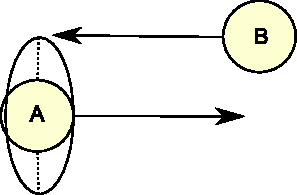
\includegraphics[width=0.40\textwidth]{image/TCGUrtoParticelle.pdf}
	\caption{Rappresenzatione schematica di un urto tra due particelle gassose.}
	\label{fig:TCG:UrtoParticelle}
\end{figure}

Il numero di urti di una particella � dato da 
\begin{equation}
	n_{urti} = \pi \cdot D^2 \cdot <v> \cdot \Delta t \cdot N
	\label{eq:UrtiParticella}
\end{equation}
mentre la frequenza di urti totali � data da:
\begin{equation}
	\frac{n_{urti TOT}}{\Delta t} = (\pi \cdot D^2 \cdot <v> \cdot N) \cdot N
	\label{eq:FreqUrtiParticella}
\end{equation}

Poich� se la particella A urta la particella B anche B urta A bisogna moltiplicare questo valore per $\frac{1}{2}$ per ottenere il numero reale di urti, inoltre poich� le particelle si muovono bisogna moltiplicare per un fattore statistico pari a $\sqrt{2}$, quindi abbiamo:
\begin{equation}
	z = \frac{\sqrt{2}}{2} \pi D^2 \cdot <v> \cdot N^2
	\label{eq:FreqUrtiParticellaZ}
\end{equation}

Se ogni urto tra due molecole � reattivo $z$ � anche la velocit� di reazione, quindi per la generica reazione 
\begin{equation}
	A\cdot + A\cdot \rightarrow A_2
	\label{eq:Reazione}
\end{equation}
e la relativa velocit� di reazione sar�:
\begin{equation}
	r = z = \frac{\sqrt{2}}{2} \pi D^2 \cdot <v> \cdot N^2 = k_{RXN} \cdot C_A^2
	\label{eq:VelocitaReazione}
\end{equation}
da cui si evince che la costante cinetica �:
\begin{equation}
	k_{RXN} = \frac{\sqrt{2}}{2} \pi D^2 \cdot <v>
	\label{eq:CostCinetica}
\end{equation}

%==============================================================================================
\section{Distribuzione della velocit� secondo Boltzman}
Affrontiamo ora la distribuzione delle velocit� molecolari come � stato fatto da Boltzman\footnote{Boltzmann, Ludwig (Vienna 1844 - Duino 1906), fisico austriaco.} nel 1869.

Indichiamo con $f_{(v)}$ la funzione di distribuzione delle velocit�, possiamo scomporla rispetto ai tre assi cartesiani, avendo cos�:
\begin{equation}
	f_{(v)} = f_{(v_x)} + f_{(v_y)} + f_{(v_z)}
	\label{eq:VelocitaScomposta}
\end{equation}

Le molecole con velocti� $\vec{v}$ compresa tra $v_x$ e $v_x + dv_x$ saranno:
\begin{equation}
	\frac{dN_{v_x}}{N} = f_{(v_x)} d v_x
	\label{eq:dNx}
\end{equation}
mentre le velocit� medie diventeranno:
\begin{equation}
	<v_x> = \frac{\int v_x dN_{v_x}}{\int dN_{v_x}} = 
					\frac{\int v_x f_{(v_x)} d v_x}{\int f_{(v_x)} d v_x} = 
	\label{eq:VelocitaMedia}
\end{equation}
essendo la velocit� data da:
\begin{equation}
	\vec{v} = \vec{i} \cdot v_x + \vec{j} \cdot v_y + \vec{k} \cdot v_z
	\label{eq:ComposizioneVelocita}
\end{equation}

consideriamo una corona sferica di spessore $d v$ e l'ipotesi di Maxwell\footnote{Maxwell, James Clerk (Edimburgo 1831 - Cambridge 1879), fisico britannico} applicata alla distribuzione di una popolazione si ha:
\begin{equation}
	d N_{v_x} \cdot d N_{v_y} \cdot d N_{v_z} = N \cdot f_{(v_x)} d v_x \cdot 
																								f_{(v_y)} d v_y \cdot 
																								f_{(v_z)} d v_z
	\label{eq:dN}
\end{equation}
e quindi 																								
\begin{equation}
	d^3 N_{v_x, v_y, v_z} = N \cdot f_{(v_x)} \cdot f_{(v_y)} \cdot f_{(v_z)} d v_x d v_y  d v_z
	\label{eq:d3N}
\end{equation}
e ancora:
\begin{equation}
	\frac{d^3 N_{v_x, v_y, v_z}}{d v_x d v_y  d v_z} = 	N \cdot f_{(v_x)} \cdot f_{(v_y)} \cdot f_{(v_z)} =
			\sigma_{(v_x, v_y, v_z)}
	\label{eq:d3N_RispettoXYZ}
\end{equation}

Poich� la $v$ � isotropa e la densit� $\sigma$ non � funzione di $\vec{v}$ ma � costante, abbiamo:
\begin{equation}
	d \sigma = 0 = N \cdot (f_{(v_x)}' \cdot f_{(v_y)} \cdot f_{(v_z)})d v_x +
								 N \cdot (f_{(v_x)} \cdot f_{(v_y)}' \cdot f_{(v_z)})d v_y +
								 N \cdot (f_{(v_x)} \cdot f_{(v_y)} \cdot f_{(v_z)}')d v_z
	\label{eq:dDensitaNullo}
\end{equation}
\begin{equation}
	d v = 0 =	v_x d v_x +	v_y d v_y +	v_z d v_z
	\label{eq:dVelocitaNullo}
\end{equation}
Dividendo tutti i membri dell'equazione \ref{eq:dDensitaNullo} per $(f_{(v_x)} \cdot f_{(v_y)} \cdot f_{(v_z)})$ e semplificando $N$ otteniamo:
\begin{multline}
	\frac {f_{(v_x)}' \cdot f_{(v_y)} \cdot f_{(v_z)}}
				{f_{(v_x)} \cdot f_{(v_y)} \cdot f_{(v_z)}} d v_x+ 
	\frac {f_{(v_x)} \cdot f_{(v_y)}' \cdot f_{(v_z)}}
				{f_{(v_x)} \cdot f_{(v_y)} \cdot f_{(v_z)}} d v_y +
	\frac {f_{(v_x)} \cdot f_{(v_y)} \cdot f_{(v_z)}'}
				{f_{(v_x)} \cdot f_{(v_y)} \cdot f_{(v_z)}}	d v_z = \\
	\frac {f_{(v_x)}'}{f_{(v_x)}} d v_x + 
	\frac {f_{(v_y)}'}{f_{(v_y)}} d v_y + 
	\frac {f_{(v_z)}'}{f_{(v_z)}} d v_z =	0
	\label{eq:dDensitaNulloDivisoFvXYZ}
\end{multline}
essendo:
\begin{align}
		f_{(v_x)}' & = \frac{\partial f_{(v_x)}}{\partial v_x} &
		f_{(v_y)}' & = \frac{\partial f_{(v_y)}}{\partial v_y} &
		f_{(v_z)}' & = \frac{\partial f_{(v_z)}}{\partial v_z} 
	\label{eq:DefinizioniDFv}
\end{align}
abbiamo:
\begin{equation}
	\frac {1}{f_{(v_x)}} \frac{\partial f_{(v_x)}}{\partial v_x} d v_x + 
	\frac {1}{f_{(v_y)}} \frac{\partial f_{(v_y)}}{\partial v_y} d v_y + 
	\frac {1}{f_{(v_z)}} \frac{\partial f_{(v_z)}}{\partial v_z} d v_z =	0
	\label{eq:dDensitaNulloDivisoFvXYZ_sostituitoDerivate}
\end{equation}

Per risolvere l'equazione cos� ottenuta si utilizza il metodo dei moltiplicatori indeterminati di Lagrange\footnote{Lagrange, Giuseppe Luigi (Torino 1736 - Parigi 1813), matematico e astronomo italiano di origine francese.}.
Moltiplichiamo le equazione \ref{eq:dVelocitaNullo} per $\lambda$ 
\begin{equation}
	d v = 0 =	v_x \cdot \lambda d v_x +	v_y \cdot \lambda d v_y +	v_z \cdot \lambda d v_z
	\label{eq:dVelocitaNulloLambda}
\end{equation}
sommiamola l'equazione appena ottenuta alla \ref{eq:dDensitaNulloDivisoFvXYZ_sostituitoDerivate} ricavando, cos�:
\begin{multline}
	\left(\frac {1}{f_{(v_x)}} \frac{\partial f_{(v_x)}}{\partial v_x} + v_x \cdot \lambda \right) d v_x + 
	\left(\frac {1}{f_{(v_y)}} \frac{\partial f_{(v_y)}}{\partial v_y} + v_y \cdot \lambda \right) d v_y + \\
	\left(\frac {1}{f_{(v_z)}} \frac{\partial f_{(v_z)}}{\partial v_z} + v_z \cdot \lambda \right) d v_z = 0
	\label{eq:dDensitaNulloDivisoFvXYZ_sostituitoDerivate}
\end{multline}
L'equazione cos� ottenuta risulta soddisfatta se tutti i tre membri nelle parentesi risultano nulli:
\begin{multline}
	\frac {1}{f_{(v_x)}} \frac{\partial f_{(v_x)}}{\partial v_x} + v_x \cdot \lambda = 0\\
	\frac {1}{f_{(v_x)}} \frac{\partial f_{(v_x)}}{\partial v_x} = - v_x \cdot \lambda \\
	\frac {1}{f_{(v_x)}}d f_{(v_x)} = - v_x \cdot d v_x \lambda \\
	ln \left(f_{(v_x)}\right) = - \frac{\lambda}{2} \cdot v_x^2 + C\\
	f_{(v_x)} = e^{- \frac{\lambda}{2} \cdot v_x^2 + C} = \alpha \cdot e^{- \frac{\lambda}{2} \cdot v_x^2}
	\label{eq:SoluzEquazMoltiplicLagrange}
\end{multline}
Bisogna ora determinare le due costanti $\alpha$ e $\lambda$; ricordando l'equazione \ref{eq:dNx}, integrata risulta:
\begin{equation}
	\int_{-\infty}^\infty dN_{v_x} = \int_{-\infty}^\infty  f_{(v_x)} d v_x = \int_{-\infty}^\infty \alpha \cdot e^{- \frac{\lambda}{2} \cdot v_x^2} dv_x
	\label{eq:dNxIntegrata}
\end{equation}
la cui soluzione porta a determinare $\alpha=\sqrt{\frac{\lambda}{\pi}}$

Come seconda condizione al contorno si ricorda l'equazione dell'energia cinetica di un gas (equazione \ref{eq:EnergCientica}) dove la $<v_x^2>$ deriva dall'equazione \ref{eq:VelocitaMedia}:
\begin{equation}
	<v_x^2> = \frac	{\int_0^\infty v_x^2 f_{(v_x)} d v_x}
									{\int_0^\infty f_{(v_x)} d v_x} =
						\frac	{\frac{1}{4}\sqrt{\frac{\pi 2^3}{\lambda^3}}}
									{\frac{1}{2}\sqrt{\frac{\pi 2}{\lambda}}} = \frac{1}{\lambda}
	\label{eq:VelocitaMediaIntegrata}
\end{equation}
Poich� la velocit� media quadratica � pari a:
\begin{equation}
	<v^2> = <v_x^2> + <v_y^2> + <v_z^2> 
				= \frac{1}{\lambda} + \frac{1}{\lambda} + \frac{1}{\lambda} 
				= \frac{3}{\lambda}
	\label{eq:ValoreVRispettoLambda}
\end{equation}
Considerando un'unica molecola, per l'equazione \ref{eq:EnergCientica} abbiamo:
\begin{equation}
	<v^2> = \frac{3 \cdot K_B \cdot T}{m}
	\label{eq:EnergiaCineticaParticella}
\end{equation}
che inserita nell'equazione \ref{eq:ValoreVRispettoLambda} ci porta a ricavare $\lambda$
\begin{equation}
	\frac{3}{\lambda} = <v^2> = \frac{3 \cdot K_B \cdot T}{m} \Rightarrow \lambda = \frac{m}{K_B \cdot T}
	\label{eq:Lambda}
\end{equation}
che ci permette di determinare $\alpha$:
\begin{equation}
	\alpha = \sqrt{\frac{\lambda}{\pi}} = \sqrt{ \frac{m}{K_B \cdot T} \frac{1}{\pi}}
	\label{eq:alfa}
\end{equation}

Tornando alla funzione di distribuzione delle velocit� abbiamo:
\begin{equation}
	f_{(v_x)} = \alpha \cdot e^{- \frac{\lambda}{2} \cdot v_x^2} = \sqrt{ \frac{m}{K_B \cdot T} \frac{1}{\pi}} \cdot e^{- \frac{m}{2 K_B \cdot T} \cdot v_x^2}
	\label{eq:FunzDistribVxRisolta}
\end{equation}
e, considerando le tre dimensioni:
\begin{multline}
	f_{(v_x, v_y, v_z)} = f_{(v_x)} \cdot f_{(v_y)} \cdot f_{(v_z)} =\\
											 \left(\frac{m}{\pi \cdot K_B \cdot T}\right)^\frac{3}{2} \cdot 
											 e^{- \frac{m}{2 K_B \cdot T} \cdot \left(v_x^2 + v_y^2 + v_z^2\right)} = \\
											 \left(\frac{m}{\pi \cdot K_B \cdot T}\right)^\frac{3}{2} \cdot 
											 e^{- \frac{m}{2 K_B \cdot T} \cdot v^2}
	\label{eq:FunzDistribVxyzRisolta}
\end{multline}

Essendo per definizione
\begin{equation}
	<v> = \frac{\int_0^\infty v dN_{v}}{\int_0^\infty dN_{v}} = 
					\frac{\int_0^\infty v f_{(v)} d v}{\int_0^\infty f_{(v)} d v} =
					\sqrt{\frac{8 \cdot K_B \cdot T}{\pi \cdot m}}
	\label{eq:VelocitaMediaIntegrata2}
\end{equation}
Per quanto visto precedentemente (equazione \ref{eq:FreqUrtiParticella}) la frequenza d'urto tra due particelle uguali risulter�
\begin{equation}
	z_{A-A} = \frac{\sqrt{2}}{2} \pi D_A^2 \cdot <v> \cdot N^2 =
						\frac{\sqrt{2}}{2} \pi D_A^2 \cdot \sqrt{\frac{8 \cdot K_B \cdot T}{\pi \cdot m}} \cdot N^2 = \sqrt{\frac{4 K_B T \pi}{m}} D_A^2 \cdot N^2
	\label{eq:FreqUrtiParticellaFinale}
\end{equation}
e la costante cinetica � quindi:
\begin{equation}
	K_{cin} = \frac{\sqrt{2}}{2} \pi D_A^2 \cdot \sqrt{\frac{8 \cdot K_B \cdot T}{\pi \cdot m}} 
	\label{eq:CostCinFinale}
\end{equation}

Se la reazione avviene tra due particelle differenti avremo:
\begin{equation}
	K_{cin} = \frac{\sqrt{2}}{2} \pi \left(\frac{D_A + D_B}{2}\right)^2 \cdot 
						\sqrt{\frac{8 \cdot K_B \cdot T}{\pi \cdot m_{eff}}}
	\label{eq:CostCinFinaleMolecoleDiverse}
\end{equation}
dove $D_A$ � il diametro della particella $A$, $D_B$ � il diametro della particella $B$ e $m_{eff}=\frac{m_A \cdot m_B}{m_A + m_B}$
		\chapter{Meccanica quantistica}
Dallo studio della radiazione emessa dal corpo nero Stefan\footnote{Stefan, Joseph (Sankt Peter 1835 - Vienna 1893), fisico austriaco.} e Boltzman\footnote{Boltzmann, Ludwig (Vienna 1844 - Duino 1906), fisico austriaco.} deducono la legge che prende il loro nome, secondo cui:
\begin{equation}
	M=\sigma \cdot T^4
	\label{eq:StefanBoltzman}
\end{equation}
dove \(M\) � la potenza emessa rispetto l'area che la emette, mentre \(\sigma\) � la costante di Stefan-Boltzman.

Non tutte le lunghezze d'onda sono emesse nello stesso modo, e la \(\lambda_{MAX}\) pu� essere dedotta dalla legge di Wien\footnote{Wien, Wilhelm Carl (Gaffken, Prussia 1864 - Monaco 1928), fisico tedesco.} dove:
\begin{equation}
	\lambda_{MAX} \cdot T = cost \approx 2.9 [mm K]
\end{equation}

La fisica classica cerca di spiegare l'emissione di radiazione come se il corpo nero fosse composto da un gran numero di oscillatori, ognuno dotato di frequenza propria, che sono messi vibrazione dalla temperatura, emettendo ognuno la propria frequenza caratteristica. Questa radiazione essendo ripartita tra tutte le radiazioni caratteristiche porta ad uno spettro continuo. Per la fisica classica la densit� della radiazione viene espressa dall'equazione di Rayleight\footnote{Chi era... }-Jeans\footnote{Chi era... }:
\begin{equation}
	\rho = \frac{d\epsilon}{d\lambda} = \frac{8 \pi k_B T}{\lambda^4} 
\end{equation}
Questa legge, per�, non approssima bene i dati sperimentali e soprattutto da luogo alla \textit{catastrofe ultravioletta}, ovvero:
\begin{equation}
	\underset{\lambda \rightarrow 0}{lim} \, \rho = \infty
\end{equation}

Plank\footnote{Chi era... } spiega le emissioni del corpo nero con una nuova teoria: gli oscillatori non possono variare in modo continuo la quantit� di energia emessa, ma la emettono in maniera discreta e pi� esattamente, l'enegia dipende dalla frequenza di vibrazione $\nu$ secondo la legge: secondo la legge:
\begin{equation}
	E=h \cdot \nu \cdot n
\end{equation}
dove \(h\) � la costante di Plank e \(n=1, 2, 3, \ldots\)

Da queste premesse vengono ricalcolate le emissioni del corpo nero, da cui risulta che:
\begin{equation}
	\rho = \frac{8 \pi h c}{\lambda^5} \cdot \frac{e^{-\frac{h c}{\lambda k_B T}}}{1 - e^{-\frac{h c}{\lambda k_B T}}}
\end{equation}

Nel 1929, grazie alla critica che Haisenberg\footnote{Heisenberg, Werner (W�rzburg 1901 - Monaco 1976), fisico tedesco.} muove nei confronti della meccanica classica viene formulato il principio di indeterminazione di Heisenberg secondo cui:
\begin{equation}
	\Delta p \cdot \Delta x \geq \frac {h}{2}
\end{equation}
Dove con \(\Delta p\) si � indicata la variazione della quantit� di moto della particella, mentre con \(\Delta x\) la variazione della sua posizione. \\
Come conseguenza se ne deduce che non � possibile determinare la posizione e la velocit� di una particella in un certo istante a meno di commettere un errore su una di esse tanto maggiore quanto pi� precisa � l'altra misura.

Un'altro aspetto che la fisica classica non era in grado di spiegare � l'osservazione delle righe spettrali degli atomi, che non sono continue, ma assumono valori ben definiti e interpretabili secondo l'equzione di Rydlberg\footnote{Rydberg, Robert Johannes, fisico svedese.}:
\begin{equation}
	\bar{\nu} = R_h \left( \frac{1}{2^2} - \frac{1}{n^2} \right)
\end{equation}
Con \(\bar{\nu}=\nu/c\) mentre $R_h$ � la costante di Rydlberg e $n=1, 2, 3, \ldots$.\\
Questa equazione suggerisce che le energie che un atomo pu� assumere sono ben determinate e quantizzate.

Partendo da questo presupposto Bohr\footnote{Bohr, Niels Henrik David (Copenaghen 1885-1962), fisico danese.} propone il modello atomico in cui il momento angolare degli elettroni intorno al nucleo � confinato in determinati valori e permette soltanto alcune energie, paria a:
\begin{equation}
	E_n = -\frac{\mu e^4}{8 h^2 \epsilon^2_0 n^2}
\end{equation}
in cui indichiamo con \(\mu\) la massa ridotta, pari a:
\begin{equation}
	\frac{1}{\mu}= \frac{1}{m_e} - \frac{1}{m_n}
\end{equation}
Dove \(m_e\) indica la massa degli elettroni e \(m_n\) la massa del nucleo.

%===================================================================================================
\section{Operatori e le loro propriet�}

L'operatore matematico � il simbolo di un procedimento che produce un cambiamento (fusione) in un certo oggetto.

Dato un operatore \(\Omega\) e una funzione \(f_{(x)}\) si dice che \(f_{(x)}\) � autofunzione di \(\Omega\) con autovalore \(\lambda\) se � vero:
\begin{equation}
	\Omega\left( f_{(x)} \right) = \lambda \cdot f_{(x)}
\end{equation}

Per esempio consideriamo:
\begin{align}
	\Omega = \left( \frac{d}{dx} \right) \\
	f_{(x)} = e^{\alpha x}
\end{align}
da cui si evince:
\begin{equation}
	\Omega \left( f_{(x)} \right) = \frac{d}{dx} \left( e^{\alpha x} \right) = \alpha e^{\alpha x}
\end{equation}
Dove l'autovalore \(\lambda\) � pari a \(\alpha\).

Tra i principali operatori ricordiamo:
\begin{itemize}
	\item Operatore di moltiplicazione per una costante \(c \cdot \)
	\item Operatore di elevazione al quadrato \(\left(\,\right)^2\)
	\item Operatore di derivazione \(\frac{d}{dx}\)
	\item Operatore di commutazione \(\left[ A , B \right]\) con \(A\) e \(B\) operatori. \\
				Questo operatore indica il grado di simmetria tra gli operatori \(A\) e \(B\) e viene determinato come 
				\begin{equation}
					\left[ A , B \right] = AB - BA
				\end{equation}
\end{itemize}
Un operatore � lineare se � verificato:
\begin{equation}
	\Omega\left(f_{(x)} \cdot g_{(x)}\right) = \Omega\left(f_{(x)} \right) + \Omega\left( g_{(x)}\right)
\end{equation}
e anche 
\begin{equation}
	\Omega\left(k \cdot f_{(x)} \right) = k \cdot \Omega\left(f_{(x)} \right)
\end{equation}

%===================================================================================================
\section{Assiomi della quantomeccanica}
\subsection{La funzione d'onda}
Lo stato di un sistema � completamente descritto da una funzione detta funzione d'onda, descritta come:
\begin{equation}
	\Psi=\Psi \left( x_1, y_1, z_1, \ldots, x_n, y_n, z_n, \sigma_1, \sigma_2, \ldots , \sigma_n, t  \right)
\end{equation}
dove

	\( x_n, y_n, z_n = \) Posizione della particella \(n\)
	
	\( \sigma_n = \)			Spin della particella \(n\)
	
	\( t = \) 						tempo\\
La risoluzione della funzione d'onda porta a determinare i numeri quantici.

\subsection{Gli osservabili}
Gli osservabili sono rapresentati da operatori che soddisfano le seguenti operazioni di commutazione:
\begin{equation}
	\left[ q , p_{q^I} \right] = i \hbar \delta_{q q^I} 	\:\:
 				\begin{cases}
					\delta_{q q^I} = 0	& \forall \: q \neq q^I \\
					\delta_{q q^I} = 1	& \forall \: q = q^I
				\end{cases}
\end{equation}
\begin{equation}
	\left[ q , q^I \right] = 0
\end{equation}
\begin{equation}
	\left[ p_q , p_{q^I} \right] = 0 	
\end{equation}
Dove \(q\) e \(q^I\) indicano una delle coordinate spaziali mentre \(p_q\) e \(p_{q^I}\) i corrispondenti momenti.\\
Questa propriet� non � dimostrabile ne derivabile dagli altri assiomi, e tra gli osservabili � escluso lo spin.

\subsection{Il valore medio}
Il valore medio dell'osservabile \(\Omega\) � definito come:
\begin{equation}
	<\Omega> = \frac{\int{\Psi^*\Omega^{OP}\Psi d\tau}}{\int{\Psi^*\Psi d\tau}}
\end{equation}

\subsection{La probabilit�}
La probabilit� che una particella si trovi in un elemento di volume \(d \tau\) � proporzinale a \( \left|\Psi_{(r)}\right|^2 d\tau \)

\subsection{L'equazione di Schr\"odinger}
La funzione d'onda evolve nel tempo in accordo con l'equazione
\begin{equation}
	H \Psi = i \hbar \frac{\partial \Psi}{\partial t}
	\label{eq:SchTimDip}
\end{equation}
chiamata equazione di Schr\"odinger\footnote{Schr�dinger, Erwin (Vienna 1887-1961), fisico teorico austriaco.} dipendente dal tempo.
L'operatore \(H\) � l'hamiltoniano e rappresenta l'energia totale del sistema. Viene espresso come la somma dell'energia cinetica (T) e potenziale (V) delle particelle considerate.
\begin{equation}
	H = T + V
	\label{eq:OpHamilt}
\end{equation}


%===================================================================================================
\section{L'equazione di Schr\"odinger}
Per una particella di massa \(m\) l'energia cinetica �
\begin{equation}
	T = \frac{1}{2 m}p^2 = \frac{1}{2 m}\left( p_x^2 + p_y^2 + p_z^2 \right)
	\label{eq:ECinetica}
\end{equation}
essendo, per definizione
\begin{equation}
	p_x = \frac{\hbar}{i} \cdot \frac{\partial}{\partial x}
\end{equation}
la sua elevazione al quadrato
\begin{equation}
	p_x^2 = - \hbar^2 \cdot \frac{\partial^2}{\partial x^2}
\end{equation}
e anche 
\begin{equation}
	T = -\frac{\hbar^2}{2 m} \cdot  \frac{\partial^2}{\partial x^2}
	\label{eq:EnCinMono}
\end{equation}
da cui, estenendo sulle tre dimensioni:
\begin{equation}
	p^2 = p_x^2 + p_y^2 + p_z^2 = 
				- \hbar^2 \cdot \left(\frac{\partial^2}{\partial x^2} 
				+ \frac{\partial^2}{\partial y^2} 
				+ \frac{\partial^2}{\partial z^2}\right) 
				= - h \cdot \nabla^2
\end{equation}
Quindi l'equazione \ref{eq:ECinetica} risulta essere:
\begin{equation}
	T = -\frac{\hbar^2}{2 m} \cdot \nabla^2
	\label{eq:EnCinet}
\end{equation}
E l'equazione di Schr\"odinger ( \ref{eq:SchTimDip} ) considerando l'equazione \ref{eq:OpHamilt} e \ref{eq:EnCinet} diventa: 
\begin{equation}
	i \hbar \frac{\partial\Psi}{\partial t} = - \frac{\hbar^2}{2 m} \nabla^2\Psi + V \Psi
\end{equation}

%===================================================================================================
\section{L'equazione di Schr\"odinger indipendente dal tempo}
Se l'enerigia potenziale � indipendente dal tempo � possibile semplificare l'equazione di Schr\"odinger ponendo:
\begin{equation}
	\Psi_{(\vec{r}, \vec{\sigma}, t)} = \Phi_{(\vec{r}, \vec{\sigma})} \cdot g_{(t)}
\end{equation}
quindi
\begin{equation}
	H\left(\Phi \cdot g\right) = i \hbar \frac{\partial \Phi g}{\partial t} = 
															i \hbar \Phi \frac{\partial g}{\partial t}
	\label{eq:SchSost}
\end{equation}
e anche, ricordando l'equazione \ref{eq:EnCinet} dell'energia cinetica:
\begin{equation}
	i \hbar \Phi \frac{\partial g}{\partial t} = 
	-\frac{\hbar^2}{2 m} \nabla^2 \left(\Psi \cdot g \right) + V \left( \Psi \cdot g \right) =
	-\frac{\hbar^2}{2 m} \cdot g \nabla^2 \Psi + V \left( \Psi \cdot g \right)
	\label{eq:SchSostT}
\end{equation}
Dividendo ambo i membri per $\Phi \cdot g$ otterremmo:
\begin{equation}
	i \hbar \frac{1}{g} \frac{\partial g}{\partial t} = 
	-\frac{\hbar^2}{2 m} \frac{1}{\Psi } \nabla^2 \Psi + V
	\label{eq:SchSostTDivPhiG}
\end{equation}
Poich� il membro di sinistra dipende solo dal tempo $t$, mentre quello di destra dipende dalla posizione entrambi i membri devono essere uguali ad una costante ($E$).
Si ottengono cos� due equazioni, una dipendente dalla posizione e l'altra dipendente dal tempo:
\begin{equation}
	- \frac{\hbar^2}{2 m}\frac{1}{\Phi} \cdot \nabla^2 \Phi + V = E
	\label{eq:EqSchTimeIndip}
\end{equation}
\begin{equation}
	i \hbar \frac{\partial g}{\partial t} = E \cdot g
	\label{eq:EqSchTime}
\end{equation}
Dove si � indicato con \(E\) la costante.
Dall'equazione \ref{eq:EqSchTime}, separando le variabili, otteniamo:
\begin{equation}
	\frac{i \hbar }{g} dg = E dt
	\label{eq:EqSchTimeRis}
\end{equation}
che integrata permette di avere
\begin{equation}
	g_{(t)} = g_{(0)} \cdot e^{\frac{E}{i \hbar} t}
	\label{eq:EqSchTimeFin}
\end{equation}
mentre l'equazione di Schr\"odinger indipendente dal tempo (equazione \ref{eq:EqSchTimeIndip}) risulta essere:
\begin{equation}
	- \frac{\hbar^2}{2 m} \nabla \Phi + V \Phi = H \Phi = E \Phi 
	\label{eq:EqSchTimeIndPhi}
\end{equation}
Poich� consideriamo l'equazione indipendente dal tempo possiamo scriverla anche come:
\begin{equation}
	H \Psi = E \Psi 
	\label{eq:EqSchTimeInd}
\end{equation}
Applicandola al caso di atomo di idrogeno e ponendo l'origine delle coordinate spazieli del centro del nucleo otterremmo:
\begin{equation}
	- \frac{\hbar^2}{2 m} \nabla^2 \Phi - \frac{e_{-}^2}{4 \pi \epsilon_0 \vec{r}} \Phi = E \Phi
	\label{eq:EqSchTimeIndIdrogeno}
\end{equation}
Essendo l'energia potenziale:
\begin{equation}
	V = - \frac{e_{-}^2}{4 \pi \epsilon_0 \vec{r}}
	\label{eq:EnPotIdrogeno}
\end{equation}
Dove \(\vec{r}\) indica la distanza dal centro del nucleo, mentre $e_-$ la carica dell'elettrone.

%===================================================================================================
\section{Particella in una scatola di potenziale monodimensionale}
Consideriamo una particella il cui movimento sull'asse $x$ � compresa tra $0$ e $L$. All'interno della scatola l'energia potenziale $(V$) assume valore nullo, mentre all'esterno assume $\infty$, come rappresentato in \figurename~\ref{fig:MQ:ScatolaPotenziale}.
\begin{figure}[htbp]
	\centering
	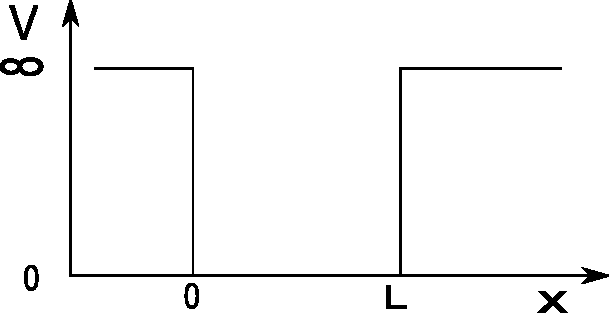
\includegraphics[width=0.60\textwidth]{image/MQScatolaPotenziale.pdf}
	\caption{Andamento dell'energia potenziale lungo l'asse x}
	\label{fig:MQ:ScatolaPotenziale}
\end{figure}

L'equazione di Schr\"odinger indipendente dal tempo (\ref{eq:EqSchTimeInd}) diventa, essendo l'energia potenziale nulla:
\begin{equation}
	H \Phi = E \Phi = T \Phi + V \Phi = T \Phi 
	\label{eq:EqSchTimeIndScatPot}
\end{equation}
quindi per quando visto precedentemente (equazione \ref{eq:EnCinMono}) potremmo scrivere l'equazione \ref{eq:EqSchTimeIndScatPot} come:
\begin{equation}
	E \Phi = T \Phi = - \frac{\hbar^2}{2 m} \cdot \frac{\partial^2 \Phi}{\partial x^2}
	\label{eq:EqSchTimeIndScatPot2}
\end{equation}
e anche:
\begin{equation}
	\frac{\partial^2 \Phi}{\partial x^2} +  \frac{2 m E}{\hbar^2} \Phi = 0 
	= \frac{\partial^2 \Phi}{\partial x^2} +  k^2 \Phi
	\label{eq:EqSchTimeIndScatPotVarSep}
\end{equation}
dove si � posto
\begin{equation}
	k^2= \frac{2 m E}{\hbar^2}
	\label{eq:DefinizK}
\end{equation}

L'equazione \ref{eq:EqSchTimeIndScatPotVarSep} pu� essere risolta ponendo
\begin{equation}
	\Phi = A cos(k x) + B sin(k x)
	\label{eq:EquazPhiScatPot}
\end{equation}
e considerando le condizioni ai limiti della scatola, ovvero:
\begin{align}
	\Phi_{(0)} & = 0 = A cos(0) + B sin(0) \\
	\Phi_{(L)} & = 0 = A cos(k L) + B sin(k L)
	\label{eq:EquazPhiLimitScatPot}
\end{align}
si nota che poich� la prima equazione � verificata se $A = 0$ la seconda si riduce a 
\begin{equation}
	\Phi_{(L)} = 0 = B sin(k L)
	\label{eq:EquazPhiLimitScatPotSemplif}
\end{equation}
Essendo \(B \neq 0\) l'equazione \ref{eq:EquazPhiLimitScatPotSemplif} � verificata se \(k L = n \pi\) da cui si evince, ricordando il significato di $k$ riportato nell'equazione \ref{eq:DefinizK}:
\begin{equation}
	\sqrt{\frac{2 m E}{\hbar^2}} L = n \pi
	\label{eq:SoluzScatPot}
\end{equation}
che risolta rispetto a \(E\) porta a:
\begin{equation}
	\frac{2 m E}{\hbar^2} L^2 = n^2 \pi^2
	\label{eq:SoluzQuadScatPot}
\end{equation}
\begin{equation}
	E = \frac{ n^2 \pi^2 \hbar^2}{L^2 2 m}
	\label{eq:SoluzEScatPot}
\end{equation}
Da cui si evidenzia che l'energia � quantizzata.

Il valore della costante \(B\) viene determinato ricordanosi che la probabilit� della particella di trovarsi nella scatola � unitaria, quindi:
\begin{multline}
	\int_0^L{\left|\Phi\right|^2dx}	= 
	B^2 \int_0^L{sin^2\left(k x \right)} dx = \\
	B^2 \int_0^L{sin^2\left(\frac{n \pi}{L} x \right)} dx =
	\left[\frac{x}{2} - \frac{sin(2 k x)}{4 k}\right]^L_0 \cdot B^2 =1
	\label{eq:IntBScatPot}
\end{multline}
che risolta
\begin{equation}	
	\left(\frac{L}{2} - \frac{sin(2 n \pi)}{4 \frac{n \pi}{L}}\right) - \left(\frac{0}{2} - \frac{sin(0)}{4 \frac{n \pi}{L}}\right) = \frac{1}{B^2} = \frac{L}{2}
	\label{eq:SoluzIntBScatPot}
\end{equation}
e quindi � evidente che:
\begin{equation}	
	B = \sqrt{\frac{2}{L}}
	\label{eq:ValBScatPot}
\end{equation}
Da cui si ottiene che 
\begin{equation}	
	\Phi_{(x)} = \sqrt{\frac{2}{L}} sin\left(\frac{n \pi}{L} x \right)
	\label{eq:PhiScatPot}
\end{equation}
e la probabilit� della particella di trovarsi nella posizione \(x\) della scatola diventa 
\begin{equation}	
	\left|\Phi_{(x)}\right|^2 = \frac{2}{L} sin^2\left(\frac{n \pi}{L} x \right)
	\label{eq:ProbScatPot}
\end{equation}

\subsection{Particella in una buca di potenziale tridimensionale}
Nel caso di una scatola tridimensionale con dimensioni \(a \times b \times c\) essendo:
\begin{equation}	
	H \Phi = E \Phi = - \frac{\hbar^2}{2 m} \cdot \left(\frac{\partial^2 \Phi}{\partial x^2} 
				+ \frac{\partial^2 \Phi}{\partial y^2} 
				+ \frac{\partial^2 \Phi}{\partial z^2}\right) 
	\label{eq:SchScatPot3D}
\end{equation}
e per simetria si ha:
\begin{equation}	
	\Phi_{(x, y, z)} = \Phi_{(x)} \cdot \Phi_{(y)} \cdot\Phi_{(z)} = \Phi_1 \cdot \Phi_2 \cdot\Phi_3
	\label{eq:SchSimmScatPot3D}
\end{equation}
Che sostituite nell'equazione \ref{eq:SchScatPot3D} porta a
\begin{equation}	
	- \frac{\hbar^2}{2 m} \cdot \left( \Phi_2 \cdot\Phi_3 \cdot \frac{\partial^2 \Phi_1}{\partial x^2} 
				+ \Phi_1 \cdot \Phi_3 \cdot \frac{\partial^2 \Phi_2}{\partial y^2} 
				+ \Phi_1 \cdot \Phi_2 \cdot \frac{\partial^2 \Phi_3}{\partial z^2}\right) = E \cdot \Phi_1 \cdot \Phi_2 \cdot\Phi_3
	\label{eq:SchScatSimmPot3D}
\end{equation}

Dividendo ambo i membri dell'equazione per \(\Phi_1 \cdot \Phi_2 \cdot\Phi_3\) otteniamo
\begin{equation}	
	- \frac{\hbar^2}{2 m} \cdot \left( \frac{1}{\Phi_1} \cdot \frac{\partial^2 \Phi_1}{\partial x^2} 
				+ \frac{1}{\Phi_2}  \cdot \frac{\partial^2 \Phi_2}{\partial y^2} 
				+ \frac{1}{\Phi_3} \cdot \frac{\partial^2 \Phi_3}{\partial z^2}\right) = E 
	\label{eq:SchSostDivScatPot3D}
\end{equation}
Ponendo \(\frac{2 m  E}{\hbar^2}= k_1 + k_2 + k_3\) e sostituendolo nell'equazione appena vista si ottiene:
\begin{equation}	
	\left( \frac{1}{\Phi_1} \cdot \frac{\partial^2 \Phi_1}{\partial x^2} + k_1^2 \right) +
	\left( \frac{1}{\Phi_2} \cdot \frac{\partial^2 \Phi_2}{\partial x^2} + k_2^2 \right) +
	\left( \frac{1}{\Phi_3} \cdot \frac{\partial^2 \Phi_3}{\partial x^2} + k_3^2 \right) = 0
	\label{eq:SchSostKDivScatPot3D}
\end{equation}

Dovendo essere ogni elemento dell'equazione \ref{eq:SchSostKDivScatPot3D} nullo si ricava, come per il caso monodimensionale:
\begin{align}	
	\Phi_1 & = \sqrt{\frac{2}{a}} sin\left(\frac{n_1 \pi}{a} x \right) \\
	\Phi_2 & = \sqrt{\frac{2}{b}} sin\left(\frac{n_2 \pi}{b} y \right) \\
	\Phi_3 & = \sqrt{\frac{2}{c}} sin\left(\frac{n_3 \pi}{c} z \right)
	\label{eq:PhiScatPot3D}
\end{align}
e quindi:
\begin{equation}	
	\Phi_{(x, y, z)} = \Phi_1 \cdot \Phi_2 \cdot\Phi_3 = 2 \cdot
		\sqrt{\frac{2}{a b c}} sin\left(\frac{n_1 \pi}{a} x \right) \cdot
		sin\left(\frac{n_2 \pi}{b} y \right) \cdot
		sin\left(\frac{n_3 \pi}{c} z \right)
	\label{eq:DefPhiScatPot3D}
\end{equation}
mentre l'energia risulta essere:
\begin{equation}	
	E^{3D} = 	\frac{n_1^2 \pi^2}{a^2} \frac{\hbar^2}{2 m} + 
						\frac{n_2^2 \pi^2}{b^2} \frac{\hbar^2}{2 m} + 
						\frac{n_3^2 \pi^2}{c^2} \frac{\hbar^2}{2 m}
	\label{eq:EScaPot3D}
\end{equation}

% ==================================================================================================
\section{Oscillatore armonico monodimensionale}
Analizziamo una particella che si muove lungo l'asse $x$ sottoposta a una forza di richiamo 
nell'origine pari a $F = -K x$; di conseguenza l'energia potenziale �:
\begin{equation}	
	V = \frac{K}{2}x^2
	\label{eq:VOscArmMono}
\end{equation}
per cui l'equazione di Schr\"odinger indipendente dal tempo (equazione \ref{eq:EqSchTimeInd}) diventa:
\begin{equation}	
	H \Psi = E \Psi = 
	T \Psi + V \Psi = 
	- \frac{\hbar}{2 m} \frac{\partial^2 \Psi}{\partial x^2} + \frac{K}{2}x^2 \Psi
	\label{eq:SchOscArmMon}
\end{equation}
Questa equazione pu� essere riarrangiata, per essere risolta pi� agevolmente, nel seguente modo:
\begin{equation}	
	\frac{\hbar^2}{2 m} \frac{\partial^2 \Psi}{\partial x^2} + \left( E - \frac{K}{2}x^2 \right) \Psi  = 0
	\label{eq:SchArrOscArmMon}
\end{equation}
Dividendo il tutto per $\frac{\hbar^2}{2 m}$ otteniamo:
\begin{equation}	
	\frac{\partial^2 \Psi}{\partial x^2} + \left( \frac{2 m E}{\hbar^2} - \frac{K m}{ \hbar^2} x^2 \right) \Psi  = 0
	\label{eq:SchDivOscArmMon}
\end{equation}
Ponendo $\alpha = \frac{2 m E}{\hbar^2}$, $\beta = \sqrt{\frac{K m}{\hbar^2}}$ e $z = \beta^{\frac{1}{2}} x$ otteniamo:
\begin{equation}	
	\frac{\partial^2 \Psi}{\partial x^2} + \left( \alpha - \beta z^2 \right) \Psi  = 0
	\label{SchRaccOscArmMon}
\end{equation}
Dividendo ambo i membri per $\beta$ otteniamo:
\begin{equation}	
	\frac{\partial^2 \Psi}{\partial \beta x^2} + \left( \frac{\alpha}{\beta} - z^2 \right) \Psi  =
	\frac{\partial^2 \Psi}{\partial z^2} + \left( \frac{\alpha}{\beta} - z^2 \right) \Psi  = 0
	\label{eq:SchDivBetaOscArmMon}
\end{equation}

Questa equazione, nel caso di $z^2>>\frac{\alpha}{\beta}$ porterebbe come soluzione a
\begin{equation}	
	\Psi = A \cdot e^{-\frac{z^2}{2}}
	\label{eq:SoluzAproxPsiOscArmMon}
\end{equation}

Per far si che questa soluzione valga anche per valori di $z$ bassi va trasformata moltiplicandola per un polinomio ($v_{(z)}$) detto polinomio modulante, quindi otteniamo:
\begin{equation}	
	\Psi = v_{(z)} \cdot e^{-\frac{z^2}{2}}
	\label{eq:SoluzPoliPsiOscArmMon}
\end{equation}
determiniamo ora il polinomio.

Iniziamo a determinare, nota la funzione di $\Psi$ dall'equazione \ref{eq:SoluzPoliPsiOscArmMon}, le sue derivate:
\begin{multline}	
	\frac{\partial \Psi}{\partial z} = 
				v_{(z)}^{'} \cdot e^{-\frac{z^2}{2}} +
				v_{(z)} \cdot \left[ -\left( \frac{2}{2} z \right) e^{-\frac{z^2}{2}} \right] = 
				v_{(z)}^{'} \cdot e^{-\frac{z^2}{2}} - v_{(z)} \cdot z \cdot e^{-\frac{z^2}{2}}
	\label{eq:Deriv1PsiOscArmMon}
\end{multline}
mentre la derivata seconda risulter� essere
\begin{multline}	
	\frac{\partial^2 \Psi}{\partial z^2} = \\
				v_{(z)}^{''} \cdot e^{-\frac{z^2}{2}} + 
				\left( -z \cdot e^{-\frac{z^2}{2}} \right) \cdot v_{(z)}^{'} -
				v_{(z)}^{'} \cdot z \cdot e^{-\frac{z^2}{2}} -
				v_{(z)} \left[ 1 \cdot e^{-\frac{z^2}{2}} - 
				z \cdot \left( -z \cdot e^{-\frac{z^2}{2}}\right) \right]	\\ = 
				v_{(z)}^{''} \cdot e^{-\frac{z^2}{2}} -
				2 \cdot v_{(z)}^{'} \cdot z \cdot e^{-\frac{z^2}{2}} -
				v_{(z)} \cdot e^{-\frac{z^2}{2}} +
				v_{(z)} \cdot z^2 \cdot  e^{-\frac{z^2}{2}}
	\label{eq:Deriv2PsiOscArmMon}
\end{multline}

Sostituendo le equazioni \ref{eq:Deriv1PsiOscArmMon} e \ref{eq:Deriv2PsiOscArmMon} nell'equazione di Schr\"odinger (\ref{eq:SchDivBetaOscArmMon}) otteniamo:
\begin{multline}	
	v_{(z)}^{''} \cdot e^{-\frac{z^2}{2}} -
	2 \cdot v_{(z)}^{'} \cdot z \cdot e^{-\frac{z^2}{2}} -
	v_{(z)} \cdot e^{-\frac{z^2}{2}} + \\
	v_{(z)} \cdot z^2 \cdot  e^{-\frac{z^2}{2}} +
	\left( \frac{\alpha}{\beta} - z^2 \right) \cdot v_{(z)} \cdot e^{-\frac{z^2}{2}} = 0
	\label{eq:SchPolModOscArmMon}
\end{multline}
che, effettuando le opportune semplificazioni, porta al seguente risultato:
\begin{equation}	
	v_{(z)}^{''} -
	2 \cdot v_{(z)}^{'} \cdot z  -
	\left( \frac{\alpha}{\beta} - 1 \right) \cdot v_{(z)}  = 0
	\label{eq:SchPolModSemplOscArmMon}
\end{equation}

indichiamo ora il polinomio $v_{(z)}$ e le sue derivate come:
\begin{align}	
	v_{(z)}  			& = \sum^{\infty}_{n=0} a_n \cdot z^n \\
	v_{(z)}^{'} 	& = \sum^{\infty}_{n=0} a_n \cdot n \cdot z^{n-1} \\
	v_{(z)}^{''} 	& = \sum^{\infty}_{n=0} a_n \cdot n \cdot (n - 1) \cdot z^{n - 2} 
	\label{eq:PolSommatorieOscArmMon}
\end{align}

Inserendo le equazioni appena viste nella \ref{eq:SchPolModSemplOscArmMon} otteniamo:
\begin{equation}	
	\sum^{\infty}_{n=0} a_n \cdot n \cdot (n - 1) \cdot z^{n - 2} -
	2 \cdot \sum^{\infty}_{n=0} a_n \cdot n \cdot z^n  -
	\left( \frac{\alpha}{\beta} - 1 \right) \cdot \sum^{\infty}_{n=0} a_n \cdot z^n  = 0
	\label{eq:SchPolSommatorieSemplOscArmMon}
\end{equation}
Raccogliendo i vari termini si ricava:
\begin{equation}	
	\sum^{\infty}_{n=0} a_n \cdot n \cdot (n - 1) \cdot z^{n - 2} -
	\sum^{\infty}_{n=0} a_n \cdot \left( - \frac{\alpha}{\beta} + 1 + 2 n \right)\cdot z^{n} = 0
	\label{eq:SchPolSommatorieRaccolteSemplOscArmMon}
\end{equation}

L'equazione scritta � verificata se i termini che moltiplicano $z^n$ e $z^{n-2}$ sono equivalenti,ed essendo le due sfalsate di 2 abbiamo:
\begin{equation}	
	a_{n+2} \cdot (n+2) \cdot ((n+2) - 1) =
	a_n \cdot \left( - \frac{\alpha}{\beta} + 1 + 2 n \right)
	\label{eq:EquivTerminiSommatoriaOscArmMon}
\end{equation}
da cui si evidenzia:
\begin{equation}
	\frac	{a_{n+2}}
				{a_{n}} = 
	\frac	{1 - \frac{\alpha}{\beta} + 2 n}
				{(n + 2) \cdot (n + 1)}
	\label{eq:EquivTerminiSommatoriaOscArmMon}
\end{equation}
Determinando il limite per $n \rightarrow \infty$ otteniamo:
\begin{equation}
	\underset{n \rightarrow \infty}{lim} \, \frac	{a_{n+2}}
				{a_{n}} = \frac{2}{n}
	\label{eq:LimiteTerminiSommatoriaOscArmMon}
\end{equation}
che � confrontabile con l'espansione in serie di potenze di:
\begin{equation}
	e^{z^2} = \sum^{\infty}_{n=0} b_n \cdot z^n
	\label{eq:EspansioneEz2OscArmMon}
\end{equation}
con $b_n = \frac{1}{n!}$.

Essendo
\begin{equation}
	\underset{n \rightarrow \infty}{lim} \, \frac	{b_{n+1}}
				{b_{n}} = \frac{1}{n}
	\label{eq:LimiteBn}
\end{equation}
da cui consegue che il polinomio $v_{(x)}$ si comporta come $e^{z^2}$ e, ricordando l'equazione \ref{eq:SoluzPoliPsiOscArmMon} abbiamo:
\begin{equation}	
	\Psi =e^{z^2} \cdot e^{-\frac{z^2}{2}} = e^{\frac{z^2}{2}} 
	\label{eq:SoluzPsiOscArmMon}
\end{equation}

Questo significherebbe che la probabilit� di trovare la particella aumenta all'aumentare della distanza,
ma essendo ci� non possibile il polinomio $v_{(x)}$ deve essere troncato.

\'E altres� evidente che se 
\begin{equation}
	1 + 2 n - \frac{\alpha}{\beta} = 0
	\label{eq:EspansioneEz2OscArmMon}
\end{equation}
allora il rapporto $\frac{a_{n+2}}{a_n}$ � nullo e quindi $v_{(x)}$ � un polinomio accettabile.
Ricordando le definizioni di $\alpha$ e $\beta$ abbiamo:
\begin{equation}
	\frac{\alpha}{\beta} = 2 n + 1 = 
			\frac{2 m E}{\hbar^2} \cdot \sqrt{\frac{\hbar^2}{K m}} = 
	 		\frac{2 E}{\hbar} \cdot \sqrt{\frac{m}{K}}
	\label{eq:AlphaSuBetaOscArmMon}
\end{equation}
da cui si vede che l'energia � quantizzata essendo:
\begin{equation}
	E = \sqrt{\frac{K}{m}} \cdot \hbar \left(n + \frac{1}{2}\right) = \nu \cdot \hbar \left(n + \frac{1}{2}\right)
	\label{eq:EOscArmMon}
\end{equation}
dove $\sqrt{\frac{K}{m}}$ � la frequenza di vibrazione $\nu$.

Nel caso di $n = 0$ abbiamo:
\begin{equation}
	E_0 = \frac{\hbar \nu }{2}
	\label{eq:EoOscArmMon}
\end{equation}
chiamata energia di punto zero (ZPE), quindi le particella non � mai ferma ma in costante movimento.

		\chapter{Termodinamica statistica}

La termodinamica statistica si occupa di collegare le propriet� macroscopiche 
della materia a quele delle particelle che la compongono. Dal punto di vista microscopico un sistema termodinamico � definito quando sono note le caratteristiche dinamiche delle particelle di cui � costituito.

Secondo la meccanica quantistica una particella pu� assumere solo una serie di valori discreti di energia, essendo queste quantizzate, e questa sar� data da:
\begin{equation}
	E = N_1 \epsilon_1 + N_2 \epsilon_2 + \dots + N_n \epsilon_n = \sum_{i=1}^{n} N_i \epsilon_i
	\label{eq:EnergiaSistema}
\end{equation}
dove $N_i$ indica il numero di particelle nello stato $i$-esimo, mentre $\epsilon_i$ le energie dello stato considerato.

Se si variano gli $N_i$, mantenendo costante la loro somma, si ottiene una serie di stati del sistema, chiamati \textsl{microstati}, la cui energia, per il microstato $E_r$, risulter� essere:
\begin{equation}
	E_r = \sum_{i=1}^{n} N_{i, r} \cdot \epsilon_i
	\label{eq:StatiSistema}
\end{equation}

Poich� il numero di particelle � molto elevato e le differenze di energia sono molto basse dal punto di vista macroscopico, l'energia si comporta come una grandezza continua.

Riassumendo, indichiamo con il termine \textsl{microstato} di un sistema termodinamico un particolare sistema caratterizzato da una particolare struttura energetica microscopica.

Indicheremo con $\Omega_{(E)}$ il numero di microstati che un sistema di energia $E$ pu� assumere; questa funzione assume un adamento caratteristico per ogni sistema, ma in generale � possibile dire che � equiparabile a:
\begin{equation}
	\Omega_{(E)} \propto E^n
	\label{eq:MicrostatiSistema}
\end{equation}
dove $n$ � il numero di particelle del sistema.

L'insieme di microstati che il sistema pu� assumere � chiamato \textit{insieme statistico} ed � rappresentativo del sistema in esame.
%==================================================================================================
\section{Postulati della termodinamica statistica}
Preso un insieme di $\aleph$ eventi, con $\aleph$ molto elevato, che si verificano in sistemi simili, la probabilit� che un particolare evento $\aleph_R$ si verifichi � espresso da:
\begin{equation}
	\omega_{R} = \underset{\aleph \rightarrow \infty}{lim} \frac{\aleph_R}{\aleph}
	\label{eq:MicrostatiSistema}
\end{equation}

Consideriamo ora un sistema chiuso in condizioni di equilibrio (quindi in uno dei micristati compatibili con l'energia posseduta); osservandolo per un tempo $\tau$ e presa una particolare grandezza $Y$, il suo valore medio � dato da:
\begin{equation}
	<Y> = \underset{\aleph \rightarrow \infty}{lim} \frac{1}{\tau} \int_0^{\tau} Y_{(t)} d t = 
				\sum_R \omega_R \cdot Y_R
	\label{eq:ValoreMedioSistema}
\end{equation}
da cui si ricava il primo pustulato, che enuncia:\\
\textsl{Il valore medio di una propriet� di un sistema termodinamico � equivalente al valore osservato mediato nel tempo.}

Questo enunciato correla i risultati ottenuti con i metodi statistici a quelli ottenuti con metodi sperimentali, mentre il secondo eneunciato, affema:\\
\textsl{In un sistema termodinamico isolato e in equilibrio tutti i suoi stati accessibili hanno la stessa probabilit�.}

L'insieme dei microstati accessibili a un sistema isolato viene chiamato \textsl{microcanonico} e, in accordo con il postulato precedente, la loro probabilit� � espressa da:
\begin{equation}
	\omega = \frac{1}{\Omega (E)}
	\label{eq:ProbabilitaMicrocanonico}
\end{equation}

%==================================================================================================
\section{Sistema a contatto con bagno termico}
Consideriamo un sistema chiuso a contatto con un bagno termico. All'equilibrio l'energia totale del sistema e ambiente � macroscopicamente costante, mentre il suo valore microscopico fluttuer� nell'intorno del suo valore medio $E_R$.

Per rappresentare il sistema si ricorre ad un insieme statistico rappresentativo, detto \textsl{canonico}, formato da un elevato numero di sistemi uguali al sistema indagato, ma che possono assumere un qualsiasi suo stato, indipendentemente dal valore energetico.

Fissiamo uno dei suoi microstati $R$ la cui energia risulta essere $E_R$; l'ambiente si trover� in uno dei suoi microstati la cui energia � $(E- E_R)$ per cui:
\begin{equation}
	\Omega(E) = \sum_r \Omega_{A}(E - E_R)
	\label{eq:MicrostatiSistemaAmbiente}
\end{equation}
ma anche, ricordando l'equazione \ref{eq:MicrostatiSistema}:
\begin{equation}
	\omega_{R} = \frac{\Omega_{A}(E - E_R)}{\Omega (E)}
	\label{eq:MicrostatiSistemaAmbiente}
\end{equation}
Essendo, per l'equazione \ref{eq:MicrostatiSistema}, $\Omega_{(E)}=C \cdot E^n$ avremo:
\begin{equation}
	\omega_{R} = \frac{C_1 \cdot (E - E_R)^{n_A}}
										{C_2 \cdot(E)^{n_{TOT}}}
	\label{eq:omegaSistema}
\end{equation}

Essendo l'ambiente molto pi� grande del sistema in esame � anche vero che $n_R << n_A$ e di conseguenza $n_A = n_{TOT} - n_R \approx n_{TOT}$ e quindi:
\begin{equation}
	\omega_{R} = \frac{C_1 \cdot (E - E_R)^{n_{TOT}}}{C_2 \cdot(E)^{n_{TOT}}} = 
							 C \cdot \left(\frac{E - E_R}{E}\right)^{n_{TOT}} = 
							 C \cdot \left( 1 - \frac{E_R}{E}\right)^{n_{TOT}}
	\label{eq:aomegaSistemaSemplificato}
\end{equation}
poich� $E_R << E$ e per $x$ che tende a $0$ � valida l'approssimazione\footnote{Infatti espandendo in serie di Taylor $e^{-x} = 1 - x - \dots$ che quindi si pu� approssimare come $e^{-x} \approx 1 - x$.} $1 - x = e^{-x}$  abbiamo:
\begin{equation}
	\omega_{R}	= C \cdot \left(e^{-\frac{E_R}{E}}\right)^{n_{TOT}}
							= C \cdot e^{-\beta E_R}
	\label{eq:omegaSistemaApprox}
\end{equation}
nota come \textsl{funzione di distribuzione canonica}. Questa equazione esprime la probabilit� del sistema di trovarsi in un particolare microstato $R$.

Essendo $\sum_R \omega_R = 1$ possiamo anche scrivere:
\begin{equation}
	\omega_{R}	= \frac{\omega_{R}}{\sum_R \omega_R} =
								\frac{C \cdot e^{-\beta E_R}}{\sum_R C \cdot e^{-\beta E_R}} = 
								\frac{e^{-\beta E_R}}{\sum_R e^{-\beta E_R}}
	\label{eq:omegaSistemaApproxTot}
\end{equation}

\section{Applicazione alla termodinamica}
Essendo l'energia totale del sistema $U$ pari alla energia media del sistema, abbiamo:
\begin{equation}
	U = \sum_R \omega_{R} \cdot E_R = \sum_R  E_R \cdot \frac{e^{-\beta E_R}}{\sum_R e^{-\beta E_R}}
	\label{eq:EnergiaTotSistema}
\end{equation}

Differenziando l'energia del sistema � evidente che:
\begin{equation}
	d U = \sum_R \omega_R d E_R + \sum_R E_R d \omega_R
	\label{eq:DifferenzialeU}
\end{equation}
dove il primo termine esprime la variazione dell'energia degli stati per mezzo di variazioni esterne (quale il volume), mentre il secondo dipende dalla redistribuzione dell'energia nei vari stati.\\
Ricordando il primo principio della termodinamica
\begin{equation}
	d U = d Q + d W
	\label{eq:PrimoPrincTermodinamica}
\end{equation}
� evidente che:
\begin{align}
	d Q & = \sum_R E_R d \omega_R \\
	d W & = \sum_R \omega_R d E_R 
	\label{eq:dQdW}
\end{align}
Introduciamo la funzione $S$ definita come 
\begin{equation}
	S = - k \sum_R \omega_R \ln \omega_R
	\label{eq:EntropiaStatistica}
\end{equation}
con $k = cost$ e, per l'equazione \ref{eq:ValoreMedioSistema} che definisce il valore medio di una variabile, $\sum_R \omega_R \ln \omega_R = <\ln \omega_R>$.

Ricordando l'equazione \ref{eq:omegaSistemaApproxTot}, e indicando con $z = \sum_R e^{-\beta E_R}$ otteniamo:
\begin{equation}
	\omega_{R}	= \frac{e^{-\beta E_R}}{\sum_R e^{-\beta E_R}} = \frac{e^{-\beta E_R}}{z}
	\label{eq:omegaSistemaApproxTotZ}
\end{equation}
Logaritmando l'equazione sopra riportata ricaviamo:
\begin{equation}
	\ln \omega_{R}	= \ln \frac{e^{-\beta E_R}}{z} = \ln e^{-\beta E_R} - \ln z = -\beta E_R - \ln z 
	\label{eq:LnOmegaSistema}
\end{equation}
ed inserendola nella \ref{eq:EntropiaStatistica} abbiamo:
\begin{equation}
	S = - k \sum_R \omega_R \ln \omega_R = 
		-k \left[ \sum_R \omega_R \left( -\beta E_R - \ln z  \right)\right] = 
		k \left(  \ln z + \beta \cdot U \right)
	\label{eq:entropiaStatisticaOmega}
\end{equation}
poich�:
\begin{align}
	- \sum_R \omega_R \ln z & = -\ln z \sum_R \omega_R = -\ln z \\
	- \beta \sum_R \omega_R \cdot E_R & = - \beta \cdot U
	\label{eq:SostituzioniEntropiaStatistica}
\end{align}

Differenziando l'espressione di S cos� ottenuta, abbiamo:
\begin{multline}
	d S = k \left[\left( \frac{\partial \ln z}{\partial \beta}\right)_{E_R} d \beta + 
								\sum_R \left( \frac{\partial \ln z}{\partial E_R}\right)_{\beta} d E_R + 
								\beta d U + U d \beta	\right] = \\
			= k \left[-\frac{\sum_R E_R e^{-\beta E_R}}{z} d \beta -
								\frac{\beta \sum_R  e^{-\beta E_R}}{z} d E_R +
								\beta d U + U d \beta	\right]
	\label{eq:DerivataEntropiaStatisticaSostituita}
\end{multline}
essendo, come ricavato precedentemente (equazione \ref{eq:EnergiaTotSistema})
\begin{equation}
	U = \sum_R  E_R \cdot \frac{e^{-\beta E_R}}{\sum_R e^{-\beta E_R}}
		= \sum_R  E_R \cdot \frac{e^{-\beta E_R}}{z}
		= \frac{\sum_R E_R \cdot e^{-\beta E_R}}{z}
	\label{eq:EnergiaTotSistema2}
\end{equation}
l'equazione di $d S$ si semplifica, diventando:
\begin{equation}
	d S = k \left[-\sum_R \left( \frac{\partial \ln z}{\partial E_R}\right) d E_R + \beta d U \right]=
				k \beta \left[ d U -	\sum_R \frac{e^{\beta E_R}}{z} d E_R \right]
	\label{eq:DerivataEntropiaStatisticaSemplificata}
\end{equation}
e per l'equazione \ref{eq:omegaSistemaApproxTotZ} anche:
\begin{equation}
	d S = k \cdot \beta \left[ d U - \sum_R \omega_R d E_R\right]
	\label{eq:DerivataEntropiaStatisticaFinale}
\end{equation}
Considerando anche l'equazione \ref{eq:dQdW} otteniamo:
\begin{equation}
	d S = k \cdot \beta \left[ d U - d W\right]
	\label{eq:DerivataEntropiaStatisticaFinale2}
\end{equation}
Per quanto noto dalla termodinamica classica:
\begin{equation}
	d S = k \cdot \beta \left[ d U -d W\right] = k \cdot \beta d Q
	\label{eq:DerivataEntropiaStatisticaEnergiaInternaSistema}
\end{equation}
Essendo noto, dal secondo principio della termodinamica, che:
\begin{equation}
	d S = \frac{d Q}{T}
	\label{eq:SecondoPrincipioTermodinamica}
\end{equation}
di conseguenza:
\begin{equation}
	\frac{d Q}{T} =  k \cdot \beta d Q
	\label{eq:DerivataEntropiaStatisticaSecondoPrincipio}
\end{equation}
e anche
\begin{equation}
	\beta = \frac{1}{k T}
	\label{eq:ValoreBeta}
\end{equation}
La costante $k$ viene ricavata analizzando un sistema di gas perfetto e vale $k_B$, ovvero la costante di Boltzman. Noto ci� � possibile scrivere:
\begin{equation}
	\omega_{R}	= \frac{e^{-\frac{E_R}{k_B T} }}{\sum_R e^{-\frac{E_R}{k_B T} }}
	\label{eq:OmegaRFinale}
\end{equation}
\begin{equation}
	z	= \sum_R e^{-\frac{E_R}{k_B T}}
	\label{eq:zFinale}
\end{equation}
\begin{equation}
	S = k_B \ln z + \frac{U}{T}
	\label{eq:SFinale}
\end{equation}
da cui si ricava l'energia libera di Helmotz:
\begin{equation}
	F = U - T S = - k_B \cdot T \cdot \ln z
	\label{eq:EnergiaHelmotz}
\end{equation}

%==================================================================================================
\section{Funzione di partizione molecolare}
Definiamo ora il significato di funzione di partizione molecolare come:
\begin{equation}
	Q = \sum e^{- \frac{\epsilon_i}{k_B T}}
	\label{eq:FunzionePartizioneMolecolare}
\end{equation}
avendo posto l'eneriga di una sola molecola come $\epsilon_i$; questo rappresenta le propriet� di una sola molecola.\\
\'E possibile esprimere anche:
\begin{equation}
	z = \sum_i \left( e^{- \frac{\epsilon_i}{k_B T}} \right) \cdot g_R
	\label{eq:zFunzionePartizioneMolecolare}
\end{equation}
dove $g_R$ indica il grado di degenerazione del sistema, ovvero quante volte un sistema in un determinato microstato � degenere. Questo parametro � particolarmente importante se consideriamo le varie particelle indistinguibili tra di loro.

Nel caso di particelle indistinguibili e non interagenti potremmo anche indicare:
\begin{equation}
	z_{indist} = \frac{Q^N}{N!}
	\label{eq:zFunzionePartizioneMolecolareIndist}
\end{equation}
mentre nel caso di particelle distinguibili avremmo:
\begin{equation}
	z_{dist} = Q^N
	\label{eq:zFunzionePartizioneMolecolareDist}
\end{equation}

L'energia di una singola particella $\epsilon_i$ pu� essere suddivisa in:
\begin{itemize}
	\item $\epsilon_{EL} = $ energia elettronica
	\item $\epsilon_{VIB} = $ energia vibrazionale
	\item $\epsilon_{ROT} = $ energia rotazionale
	\item $\epsilon_{TRAS} = $ energia traslazionale
\end{itemize}
ed essendo $\epsilon_i = \epsilon_{EL} + \epsilon_{VIB} + \epsilon_{ROT} + \epsilon_{TRAS}$ sar� anche:
\begin{equation}
	Q = \sum e^{- \frac{\epsilon_i}{k_B T}}
		= \sum e^{- \frac{\epsilon_{EL} + \epsilon_{VIB} + \epsilon_{ROT} + \epsilon_{TRAS}}{k_B T}}
		= Q_{EL} \cdot Q_{VIB} \cdot Q_{ROT} \cdot Q_{TRAS}
	\label{eq:FunzionePartizioneMolecolareEnergie}
\end{equation}
I vari contributi alla funzione di partizione molecolare vengono determinati in maniera separata.

\subsection{Contributo elettronico}
Il contributo elettronico viene determinato tramite:
\begin{equation}
	Q_{EL} =  \sum e^{- \frac{\epsilon_{EL}}{k_B T}}
	\label{eq:FunzionePartizioneMolecolareContributoElettronico}
\end{equation}
dove $\epsilon_{EL}$ � l'energia elettronica che si pu� ricavare usando l'equazione di Schr\"odinger:
\begin{equation}
	H \cdot \Psi = E_{EL} \cdot \Psi
	\label{eq:FunzPartizMolecSchrodinger}
\end{equation}
\subsection{Contributo traslazionale}
In questo caso il contributo traslazionale � ovviamente dato da;
\begin{equation}
	Q_{TRAS} =  \sum e^{- \frac{\epsilon_{TRAS}}{k_B T}}
	\label{eq:FunzionePartizioneMolecolareContributoTraslazionale}
\end{equation}
Poich�, per quanto visto precedentemente (equazione \ref{eq:EScaPot3D}), possiamo scrivere:
\begin{equation}
	\epsilon_{TRAS} = \frac {h^2}{8 m} \cdot 
										\left( \frac{n_1^2}{L^2} + \frac{n_2^2}{L^2} + \frac{n_3^2}{L^2}\right)
	\label{eq:FunzPartizMolEnergTras}
\end{equation}
con $n_1$, $n_2$ e $n_3$ che indicano i numeri quantici di moto nelle tre direzioni; si ha anche:
\begin{multline}
	Q_{TRAS} =  \sum e^{-{\frac {h^2}{8 m L^2} \cdot 
							\left( n_1^2 + n_2^2 + n_3^2\right)}\frac{1}{k_B T}} = \\
										\sum e^{- {\frac {h^2}{8 m L^2} \cdot n_1^2}\frac{1}{k_B T}}
							\cdot \sum e^{- {\frac {h^2}{8 m L^2} \cdot n_2^2}\frac{1}{k_B T}}
							\cdot \sum e^{- {\frac {h^2}{8 m L^2} \cdot n_3^2}\frac{1}{k_B T}}
	\label{eq:FunzionePartizioneMolecolareContributoTraslazionaleNumQuantici}
\end{multline}
esprimendo:
\begin{equation}
	\alpha = \left( \frac{h^2}{8 k_B \cdot T \cdot m \cdot L^2}\right)^{\frac{1}{2}}
	\label{eq:FunzPartizMolEnergTrasAlpha}
\end{equation}
Abbiamo quindi:
\begin{equation}
	Q_{TRAS} =  \sum e^{- \alpha^2 \cdot n_1^2} +
							\sum e^{- \alpha^2 \cdot n_2^2} +
							\sum e^{- \alpha^2 \cdot n_3^2}
	\label{eq:FunzionePartizioneMolecolareContributoTraslazionaleNumQuanticiAlpha}
\end{equation}
Possiamo anche, per ogni singolo $n_i$ scrivere:
\begin{equation}
	\sum e^{- \alpha^2 \cdot n_i^2} = \sum e^{- \alpha^2 \cdot n_i^2} \cdot \Delta n
	\label{eq:QtraslNiDn}
\end{equation}
essendo $\Delta n = (n + 1) - n = 1$, ma anche:
\begin{equation}
	\sum e^{- \alpha^2 \cdot n_i^2} = \sum e^{- \alpha^2 \cdot n_i^2} \cdot \Delta n \cdot \frac{\alpha}{\alpha} = \frac{1}{\alpha} \sum e^{- \alpha^2 \cdot n_i^2} \cdot \Delta n \cdot \alpha
	\label{eq:QtraslNiDnAlphaSuAlpha}
\end{equation}
Se $\alpha$ � sufficientemente piccola possiamo approssimare la sommatoria con un integrale e quindi:
\begin{equation}
	\sum e^{- \alpha^2 \cdot n_i^2} = \frac{1}{\alpha} \int_0^{\infty} e^{- \alpha^2 \cdot n_i^2} \cdot \Delta n \cdot \alpha = \frac{1}{\alpha} \int_0^{\infty} e^{- x^2} d x = \frac{1}{\alpha} \cdot \frac{\sqrt{\pi}}{2}
	\label{eq:IntQtraslNiDnAlphaSuAlpha}
\end{equation}
Da cui tornando all'equazione \ref{eq:FunzionePartizioneMolecolareContributoTraslazionaleNumQuantici} ricaviamo:
\begin{equation}
	Q_{TRAS} = \left( \frac{1}{\alpha} \cdot \frac{\sqrt{\pi}}{2} \right)^3
	\label{eq:QTrasFinaleAlpha}
\end{equation}
ed esplicitando $\alpha$ abbiamo:
\begin{equation}
	Q_{TRAS} = \left( \frac{8 k_B \cdot T \cdot m \cdot L^2}{h^2} \cdot \frac{\pi}{4} \right)^{\frac{3}{2}} = \left( \frac{2 \pi \cdot k_B \cdot T \cdot m }{h^2} \right)^{\frac{3}{2}} \cdot L^3
	\label{eq:QTrasFinale}
\end{equation}
dove $L^3 = V$ ovvero il volume.

\subsection{Contributo vibrazionale}
Come nei casi precedenti abbiamo:
\begin{equation}
	Q_{VIB} =  \sum e^{- \frac{\epsilon_{VIB}}{k_B T}}
	\label{eq:FunzionePartizioneMolecolareContributoVibrazionale}
\end{equation}
Possiamo esprimere l'energia vibrazionale considerando l'oscillatore nell'intorno di un punto, quindi:
\begin{equation}
	\epsilon_{VIB} =  \left( \frac{1}{2} + n \right) \cdot h \cdot \nu
	\label{eq:EVibOsillatoreIntornoPunto}
\end{equation}
Da cui si ricava:
\begin{equation}
	Q_{VIB} = \sum e^{- \left( \frac{1}{2} + n \right) \cdot \frac{h \cdot \nu}{k_B T}}
					= \sum e^{- \frac{1}{2} \cdot \frac{h \cdot \nu}{k_B T}} \cdot
						e^{- n \cdot \frac{h \cdot \nu}{k_B T}}
					= e^{- \frac{1}{2} \cdot \frac{h \cdot \nu}{k_B T}} \cdot
						\sum e^{- n \cdot \frac{h \cdot \nu}{k_B T}}
	\label{eq:FunzionePartizioneMolecolareContributoVibrazionaleEnergia}
\end{equation}
Dove l'ultimo passaggio � stato ottenuto essendo:
\begin{equation}
	\frac{h \cdot \nu}{2 k_B T} = cost
	\label{eq:RappCostEVib}
\end{equation}
Sviluppando la somatoria abbiamo:
\begin{equation}
	Q_{VIB} = e^{- \frac{1}{2} \cdot \frac{h \cdot \nu}{k_B T}} \cdot
						\left(  1 +
										e^{- 1 \cdot \frac{h \cdot \nu}{k_B T}} + 
										e^{- 2 \cdot \frac{h \cdot \nu}{k_B T}} +
										e^{- 3 \cdot \frac{h \cdot \nu}{k_B T}} +
										\dots	\right)
	\label{eq:QVibEspansioneSommatoria}
\end{equation}
e di conseguenza\footnote{Essendo $1 + x + x^2 + x^3 + ... = \frac{1}{1 - x}$} otteniamo:
\begin{equation}
	Q_{VIB} = e^{- \frac{h \cdot \nu}{2 k_B T}} \cdot \frac{1}{1 - e^{\frac{h \cdot \nu}{k_B T}}} =  \frac{e^{- \frac{h \cdot \nu}{2 k_B T}}}{1 - e^{\frac{h \cdot \nu}{k_B T}}}
	\label{eq:QVibFinale}
\end{equation}

\subsection{Contributo rotazionale}
Per il calcolo dell'energia rotazionale si procede in modo analogo al caso vibrazionale e il risultato finale � dato da:
\begin{equation}
	Q_{ROT} = \frac	{8 \pi^2 (2 \pi k_B T)^{\frac{3}{2}} \cdot \sqrt{I_x \cdot I_y \cdot I_z}}
									{\sigma \cdot h^3}
	\label{eq:QRotFinale}
\end{equation}
dove $I_x$, $I_y$ e $I_z$ rappresentano i tre momenti di inerzia della molecola nelle tre direzioni, mentre $\sigma$ indica il grado di simmetria della molecola.
		\chapter{Teoria dello strato di transizione}
\section{Schema di una generica reazione}
Data la  generica reazione
\begin{equation}
	A + B \rightarrow C + D
	\label{eq:ST:ReazioneGenerica}
\end{equation}
Si pu� rappresentare il processo di reazione nel seguente modo:

\begin{figure}[htbp]
	\centering
		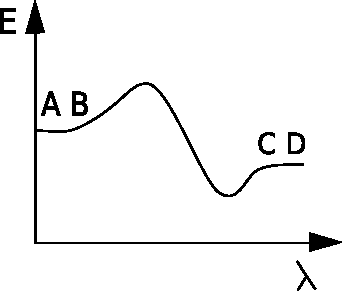
\includegraphics[height=5cm]{image/ElambdaRXN.pdf}
	\label{fig:E-lambda_RXN}
\end{figure}

dove $E$ indica l'energia, mentre $\lambda$ la coordinata di reazione.

\section{Ipotesi restrittive}
I fondatori della teoria dello stato di transizione sono Eyring\footnote{Chi era ....} e Polanyi\footnote{Polanyi, John C. (Berlino 1929), chimico canadese.} e basano le loro affermazioni sulle seguenti ipotesi:
\begin{itemize}
	\item \'E valida l'approssimazione di Born\footnote{Born, Max (Breslavia 1882 - Gottinga 1970), fisico britannico di origine tedesca.}-Hopenheimer\footnote{Dire chi era...}, ovvero: i moti elettromolecolari sono all'equilibrio ($v_{e^{-}} >> v_{nucleo}$)
	\item La distribuzione delle velocit� segue la legge di Maxwell\footnote{Maxwell, James Clerk (Edimburgo 1831 - Cambridge 1879), fisico britannico.}-Boltzman\footnote{Boltzmann, Ludwig (Vienna 1844 - Duino 1906), fisico austriaco}
	\item I sistemi che hanno superato lo stato di transizione non possono tornare indientro
	\item Vi � equilibrio tra reagenti e stato di transizione
	\item Nella prossimit� dello stato di transizione il moto lungo la coordinata di reazione � assimilabile ad una traslazione\\
		\begin{figure}[htbp]
			\centering
				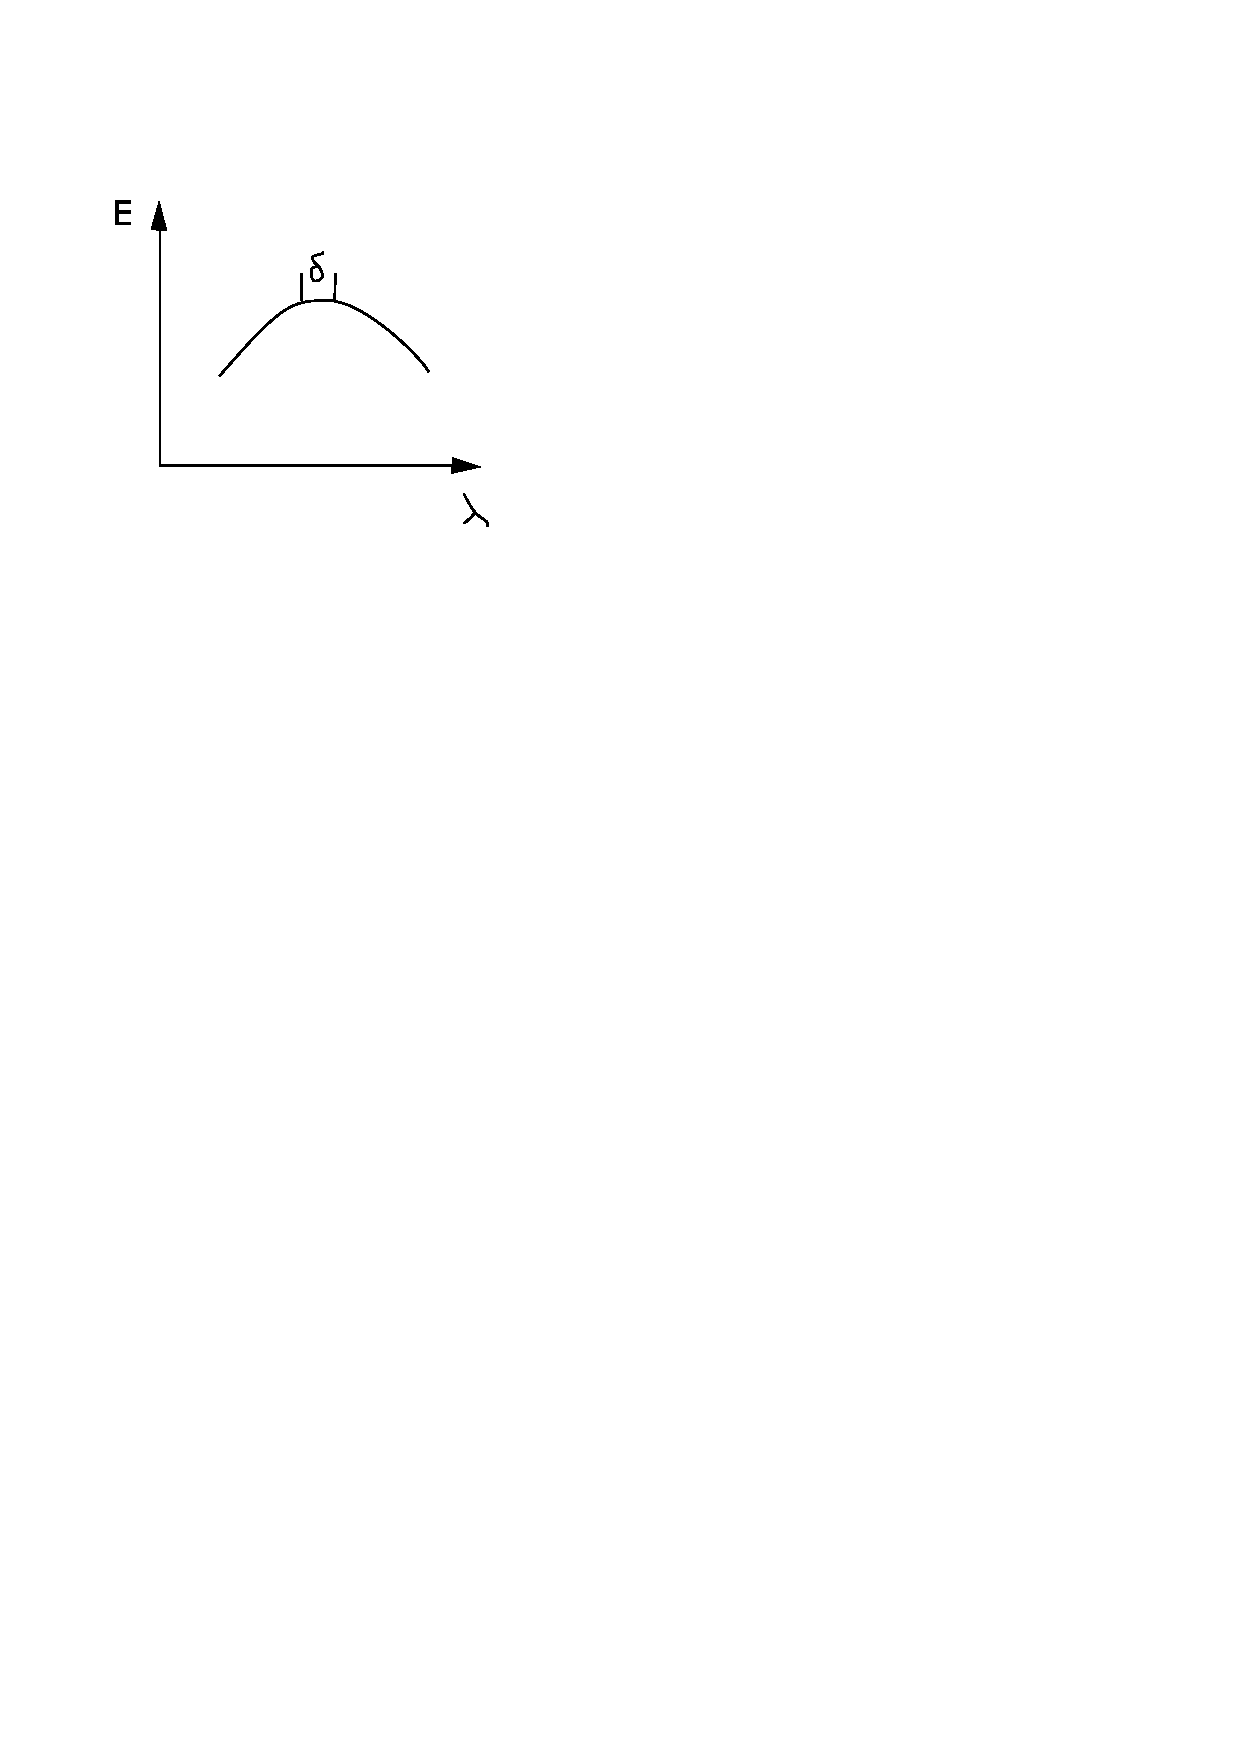
\includegraphics[height=3cm]{image/Delta_RXN.pdf}
			\label{fig:E-Delta_RXN}
		\end{figure}
\end{itemize}

Mentre la prime due ipotesi sono sempre verificate le successive sono ipotesi pi� restrittive, in particolare la terza � la pi� limitante.

\section{Velocit� di reazione}
Secondo quanto elencato qui sopra la reazione \ref{eq:ST:ReazioneGenerica} pu� essere vista come:
\begin{equation}
	A + B \rightleftharpoons X^{\ddagger} \rightarrow C + D
	\label{eq:ST:ReazioneIntermedioGenerica}
\end{equation}
Inoltre possiamo esprimere la velocit� di reazione come:
\begin{equation}
	R = C_{X^{\ddagger}} \cdot \frac{v^{\ddagger}}{\delta} \cdot \frac{1}{2}
	\label{eq:ST:VelocitaReazione}
\end{equation}
Dove $\delta$ � uno spessore arbitrario e $v^{\ddagger}$ � la velocit� della specie intermedia, che pu� essere espressa tramite la distribuzione di Boltzamn
\begin{equation}
	v^{\ddagger} = \sqrt{\frac{2 k_B \cdot T}{\pi m}}
	\label{eq:ST:VelocitaMaxwelBoltzman}
\end{equation}
che inserita nella velocit� di reazione (equazione \ref{eq:ST:VelocitaReazione}) porta a:
\begin{equation}
	R = C_{X^{\ddagger}} \cdot \frac{1}{2 \delta} \cdot \sqrt{\frac{2 k_B \cdot T}{\pi m}}
	\label{eq:ST:VelocitaReazioneMaxwelBoltzman}
\end{equation}

\subsection{Concentrazione della specie intermedia}
Cerchiamo ora di determinare $C_{X^{\ddagger}}$, sapendo che la reazione:
\begin{equation}
	A + B \rightleftharpoons X^{\ddagger}
	\label{eq:ST:ReazioneFormazioneIntermedio}
\end{equation}
si trova all'equilibrio, quindi la sua costante pu� essere espressa come:
\begin{equation}
	K_{eq} = \frac{C_{X^{\ddagger}}}{C_A \cdot C_B}
	\label{eq:ST:CostanteEquilibrioIntermedio}
\end{equation}
da cui si ottiene:
\begin{equation}
	C_{X^{\ddagger}}= K_{eq} \cdot C_A \cdot C_B
	\label{eq:ST:ConcIntermedioDaKeq}
\end{equation}
ed infine, sostituendo il risultato ottenuto nella \ref{eq:ST:VelocitaReazioneMaxwelBoltzman}, otteniamo:
\begin{equation}
	R =  K_{eq} \cdot C_A \cdot C_B \cdot \frac{1}{2 \delta} \cdot \sqrt{\frac{2 k_B \cdot T}{\pi m}}
	\label{eq:ST:VelocitaReazioneMaxwelBoltzmanKeq}
\end{equation}

\subsection{Costante di equilibrio in funzione della funzione di partizione molecolare}
Cerchiamo ora di correlare la costante di equilibrio con una funzione della \textsl{funzione di partizione molecolare}.

Ricordando dalla termodinamica che:
\begin{equation}
	G = F + P \cdot V
	\label{eq:ST:GTermodinamica}
\end{equation}
e anche 
\begin{equation}
	P \cdot V = n \cdot R \cdot T = n \cdot k_B \cdot N_A \cdot T = N \cdot k_B \cdot T
	\label{eq:ST:GasPerfetti}
\end{equation}
da questa otteniamo e dall'equazione precedente abbiamo:
\begin{equation}
	G = F +  N \cdot k_B \cdot T
	\label{eq:ST:GTermodinamicaGasPerfetti}
\end{equation}
ma dalla termodinamica statistica sappiamo che:
\begin{equation}
	F = - k_B \cdot T \cdot \ln z
	\label{eq:ST:FTermodinamicaStatistica}
\end{equation}
con $z$ \textsl{funzione di partizione}, da cui tornando all'equazione \ref{eq:ST:GTermodinamicaGasPerfetti}, ricaviamo:
\begin{equation}
	G = N \cdot k_B \cdot T - k_B \cdot T \cdot \ln z = k_B \cdot T (N - \ln z)
	\label{eq:ST:GTermodinamicaStatisticaGasPerfetti}
\end{equation}
poich�, per quanto visto precedentemente, per i gas perfetti � anche vero che:
\begin{equation}
	z = \frac{Q^N}{N!}
	\label{eq:ST:FunzParizMolecolare}
\end{equation}
otteniamo:
\begin{multline}
	G = k_B \cdot T (N - \ln \frac{Q^N}{N!}) = \\
			k_B \cdot T (N - \ln Q^N + \ln N!) =  \\
			k_B \cdot T (N - N \ln Q + N \ln N - N)
	\label{eq:ST:GFunzParizMolecolare}
\end{multline}
dove nell'ultimo passaggio � stata utilzzata l'approssimazione di Stearling\footnote{l'approssimazione di stearling dimostra che per $x$ elevati $\ln x! = x \ln x - x$}. Raccogliendo gli elementi e semplificando (considerando una sola mole di molecole) si ottiene:
\begin{multline}
	G = k_B \cdot T (N \ln N - N \ln Q) = \\
			- k_B \cdot T \cdot N (\ln Q - \ln N ) = \\
			- k_B \cdot T \cdot N \left(\ln \frac{Q}{N}\right) = \\
			- k_B \cdot T \cdot N_A \left(\ln \frac{Q}{N_A}\right) = \\
			- R \cdot T \ln \frac{Q}{N_A} 
	\label{eq:ST:GFunzParizMolecolareSemplificata}
\end{multline}

Dalla termodinamica sappiamo che:
\begin{equation}
	K_{eq} = e^{-\frac{\Delta \tilde{G}^0_R}{R \cdot T}}
	\label{eq:ST:KeqTermodinamica}
\end{equation}
dove
\begin{equation}
	\Delta \tilde{G}^0_R = \sum_i \nu_i \tilde{G}_{i\:(P,T)}
	\label{eq:ST:DGo}
\end{equation}
e dividendo ambo i membri per $R \cdot T$ ottengo:
\begin{equation}
	\frac{\Delta \tilde{G}^0_R}{R \cdot T} = \sum_i \nu_i \frac{\tilde{G}_{i\:(P,T)}}{R \cdot T}
	\label{eq:ST:DGoTR}
\end{equation}

Ricordando la definizione di $G$ ricavata prima (equazione \ref{eq:ST:GFunzParizMolecolareSemplificata}) per una mole abbiamo:
\begin{equation}
	\frac{\Delta \tilde{G}}{R \cdot T} = - \ln \frac{Q}{N_A}
	\label{eq:ST:GSuRTMoleTermoStat}
\end{equation}
da cui, inserendolo nell'equazione \ref{eq:ST:KeqTermodinamica} e logaritmando:
\begin{multline}
	\ln K_{eq} = - \frac{\Delta \tilde{G}^0_R}{R \cdot T} = 
							 - \sum_i \nu_i \frac{\tilde{G}_{i\:(P,T)}}{R \cdot T} = 
							 \sum_i \nu_i \ln\frac{Q}{N_A} = \\
							 \sum_i \ln \left(\frac{Q}{N_A}\right)^{\nu_i} = 
							 \ln \prod_i \left(\frac{Q}{N_A}\right)^{\nu_i}
	\label{eq:ST:LnKeqTermodinamicaStatistica}
\end{multline}
ed elevando ad esponente
\begin{equation}
	K_{eq} = \prod_i \left(\frac{Q}{N_A}\right)^{\nu_i}
	\label{eq:ST:LnKeqTermodinamicaStatistica}
\end{equation}

Ricordando dalla termodinamica statistiche il valore di $Q_{TRAS}$, sappiamo che:
\begin{equation}
	 Q_i = Q' \cdot V
	\label{eq:ST:QVTermoStat}
\end{equation}
quindi la costante di equilibrio risulter� essere:
\begin{equation}
	 K_{eq} = \prod \left( \frac{Q' \cdot V}{N_A} \right)^{\nu} = \prod (Q' \cdot \tilde{v})^{\nu}
	\label{eq:ST:KeqQV}
\end{equation}
essendo anche:
\begin{equation}
	 C_{TOT} = \frac{1}{\tilde{v}}
	\label{eq:ST:Ctot}
\end{equation}
abbiamo:
\begin{equation}
	K_{eq} = 	\frac{1}{C_{TOT}^{\sum_i \nu_i}} \prod_i Q'^{\nu_i} = 
						\prod_i \left( \frac{C_i}{C_0} \right)^{\nu_i} = 
						 \left( \frac{\prod_i C_i^{\nu_i}}{C_0^{\sum_i \nu_i}} \right)
	\label{eq:ST:KeqQCtot}
\end{equation}
e semplificando:
\begin{equation}
	\frac{\prod_i C_i^{\nu_i}}{C_0^{\sum_i \nu_i}} =
	\frac{\prod_i Q'^{\nu_i}}{C_{TOT}^{\sum_i \nu_i}}
	\label{eq:ST:KeqQCtotSemplif}
\end{equation}
da cui ottengo:
\begin{equation}
	\prod_i C_i^{\nu_i} =	\prod_i Q'^{\nu_i}
	\label{eq:ST:QCi}
\end{equation}
Ritornando all'equazione \ref{eq:ST:VelocitaReazioneMaxwelBoltzmanKeq} ottengo:
\begin{equation}
	R = C_A \cdot C_B \cdot \prod_i Q'^{\nu_i} \cdot \frac{1}{2 \delta} \cdot \sqrt{\frac{2 k_B \cdot T}{\pi m}}
	\label{eq:ST:VelocitaReazioneFinale}
\end{equation}
Da cui si evidenzia che la costante cinetica risulter� essere paria a:
\begin{equation}
	K_{CIN} = \prod_i Q'^{\nu_i} \cdot \frac{1}{2 \delta} \cdot \sqrt{\frac{2 k_B \cdot T}{\pi m}} = 
						\frac{1}{2 \delta} \cdot \sqrt{\frac{2 k_B \cdot T}{\pi m}} \cdot \frac{Q'_{\ddagger}}{Q_A \cdot Q_B}
	\label{eq:ST:VelocitaReazioneFinaleQ}
\end{equation}

\section{La costante cinetica}
Come si pu� vedere la costante cinetica dipende ancora dal parametro $\delta$ che essendo un parametro arbitrario deve essere rimosso. Per fare questo esplicitiamo $Q'_{\ddagger}$ ottenendo:
\begin{equation}
	K_{CIN} = \frac{1}{2 \delta} \cdot \sqrt{\frac{2 k_B \cdot T}{\pi m}} \cdot
						\frac{Q_{ROT}^{\ddagger} \cdot Q_{VIB}^{\ddagger} \cdot 
									Q_{TRAS}^{\ddagger} \cdot Q_{EL}^{\ddagger}}
								 {Q_A \cdot Q_B}
	\label{eq:ST:KcinFinaleQddagger}
\end{equation}
Il moto vibrazionale lungo la direzione delle coordinate di reazione degenera in un moto traslatorio, quindi otteniamo:
\begin{equation}
	K_{CIN} = \frac{1}{2 \delta} \cdot \sqrt{\frac{2 k_B \cdot T}{\pi m}} \cdot
						\frac{Q_{ROT}^{\ddagger}  \cdot Q_{EL}^{\ddagger} \cdot
									Q_{TRAS}^{\ddagger} \cdot (Q_{VIB-1}^{\ddagger} \cdot Q_{TRAS}^{\ddagger 1D})}
								 {Q_A \cdot Q_B}
	\label{eq:ST:KcinQddaggerDegenerato}
\end{equation}
ed essendo:
\begin{equation}
	Q_{TRAS}^{\ddagger 1D} = \sqrt{\frac{2 \pi m \cdot k_B \cdot T}{h^2}} \cdot L
	\label{eq:ST:Qdagger1D}
\end{equation}
ponendo $L = \delta$ e semplificando, otteniamo:
\begin{multline}
	K_{CIN} = \frac{1}{2} \cdot \sqrt{\frac{2 k_B \cdot T}{\pi m}} \cdot
						\sqrt{\frac{2 \pi m \cdot k_B \cdot T}{h^2}} \cdot
						\frac{Q_{ROT}^{\ddagger}  \cdot Q_{EL}^{\ddagger} \cdot
									Q_{TRAS}^{\ddagger} \cdot Q_{VIB-1}^{\ddagger}}
								 {Q_A \cdot Q_B} = \\
						\frac{k_B \cdot T}{h} \cdot
						\frac{Q_{ROT}^{\ddagger}  \cdot Q_{EL}^{\ddagger} \cdot
									Q_{TRAS}^{\ddagger} \cdot Q_{VIB-1}^{\ddagger}}
								 {Q_A \cdot Q_B}
	\label{eq:ST:KcinQddaggerDegenerato}
\end{multline}
La costante cinetica pu� anche essere esplicitata come:
\begin{multline}
	K_{CIN} =	\frac{k_B \cdot T}{h} \cdot
						\frac{Q_{ROT}^{\ddagger}  \cdot Q_{EL}^{\ddagger} \cdot
									Q_{TRAS}^{\ddagger} \cdot Q_{VIB-1}^{\ddagger}}
								 {Q_{ROT}^A  \cdot Q_{EL}^A \cdot	Q_{TRAS}^A \cdot Q_{VIB}^A \cdot 
									Q_{ROT}^B  \cdot Q_{EL}^B \cdot	Q_{TRAS}^B \cdot Q_{VIB}^B }
	\label{eq:ST:KcinEsplicitata}
\end{multline}
da cui raccogliendo i contributi elettronici:
\begin{multline}
	K_{CIN} =	\frac{k_B \cdot T}{h} \cdot
						\frac{Q_{ROT}^{\ddagger} \cdot Q_{TRAS}^{\ddagger} \cdot Q_{VIB-1}^{\ddagger}}
								 {Q_{ROT}^A \cdot	Q_{TRAS}^A \cdot Q_{VIB}^A \cdot 
									Q_{ROT}^B \cdot	Q_{TRAS}^B \cdot Q_{VIB}^B } \cdot
						\frac{Q_{EL}^{\ddagger}}{Q_{EL}^A \cdot	Q_{EL}^B} = \\
						\frac{k_B \cdot T}{h} \cdot
						\frac{Q_{ROT}^{\ddagger} \cdot Q_{TRAS}^{\ddagger} \cdot Q_{VIB-1}^{\ddagger}}
								 {Q_{ROT}^A \cdot	Q_{TRAS}^A \cdot Q_{VIB}^A \cdot 
									Q_{ROT}^B \cdot	Q_{TRAS}^B \cdot Q_{VIB}^B } \cdot
						e^{-\frac{\epsilon_{EL}^{\ddagger} - \epsilon_{EL}^A - \epsilon_{EL}^B}{k_B \cdot T}} =\\
						\frac{k_B \cdot T}{h} \cdot
						\frac{Q_{ROT}^{\ddagger} \cdot Q_{TRAS}^{\ddagger} \cdot Q_{VIB-1}^{\ddagger}}
								 {Q_{ROT}^A \cdot	Q_{TRAS}^A \cdot Q_{VIB}^A \cdot 
									Q_{ROT}^B \cdot	Q_{TRAS}^B \cdot Q_{VIB}^B } \cdot
						e^{-\frac{\Delta \epsilon_{EL}}{k_B \cdot T}}
	\label{eq:ST:KcinEsplicitataElettronici}
\end{multline}
Raccogliendo anche le $Q_{VIB}$ possiamo scrivere:
\begin{equation}
	\frac{Q_{VIB}^{\ddagger}}{Q_{VIB}^A \cdot Q_{VIB}^B} = 
	e^{- \frac{\sum \frac{h \nu^{\ddagger}}{2} - \sum \frac{h \nu^A}{2} - \sum \frac{h \nu^B}{2}}
						{k_B \cdot T}}
	\label{eq:ST:QVibrazRaccolte}
\end{equation}
l'esponente viene chiamato \textsl{$\Delta$ZPE\footnote{Zero Point Energy}} ovvero � l'energia che tutte le molecole possiedono allo stato $0$. La costante cinetica pu� essere riscritta, quindi, come:
\begin{equation}
	K_{CIN} =	\frac{k_B \cdot T}{h} \cdot
						\frac{Q_{ROT}^{\ddagger} \cdot Q_{TRAS}^{\ddagger}}
								 {Q_{ROT}^A \cdot	Q_{TRAS}^A \cdot Q_{ROT}^B \cdot Q_{TRAS}^B} \cdot
						e^{-\frac{\Delta(\epsilon_{EL} + ZPE)}{k_B \cdot T}}
	\label{eq:ST:KcinFin}
\end{equation}

Se confrontiamo l'equazione ottenuta con l'equazione di Arrenus si nota che le due equazioni sono identiche se si pone:
\begin{equation}
	\Delta E_{ATT} = \Delta(\epsilon_{EL} + ZPE)
	\label{eq:ST:ArreniusDEatt}
\end{equation}
\begin{equation}
	A = \frac{k_B \cdot T}{h} \cdot
			\frac{Q_{ROT}^{\ddagger} \cdot Q_{TRAS}^{\ddagger}}
					 {Q_{ROT}^A \cdot	Q_{TRAS}^A \cdot Q_{ROT}^B \cdot Q_{TRAS}^B}
	\label{eq:ST:ArreniusA}
\end{equation}
ottenendo quindi:
\begin{equation}
	K_{CIN} =	A \cdot e^{-\frac{\Delta E_{ATT}}{k_B \cdot T}}
	\label{eq:ST:KcinFin}
\end{equation}
		\chapter{Reazioni in fase condensata}
Le sostanze reagenti non si trovano sempre come le uniche specie presenti e, soprattutto nelle reazioni tra fasi condensate, � spesso presente una sostanza (\textsl{solvente}) che interagisce con esse. 

Gli effetti del solvente possono essere raggruppati in:
\begin{itemize}
	\item \textsl{Effetto cella}: il solvente si dispone in maniera ordinata intorno ai reagenti.
	\item \textsl{Effetto ionizzante}: si formano i cationi perch� stabilizzati dalla cella di solvente.
	\item \textsl{Solvatazione}: effetti di interazione tra solvente e soluto.
\end{itemize}
Consideriamo la generica reazione:
\begin{equation}
	X^- + CH_3Y \rightarrow XCH_3 + Y^-
	\label{eq:sol:RxnGenerica}
\end{equation}
possiamo diagrammare l'andamento secondo le coordinate di reazione (Figura \ref{fig:ELambda_Rxn_XCH3Y}),
\begin{figure}[htbp]
	\centering
		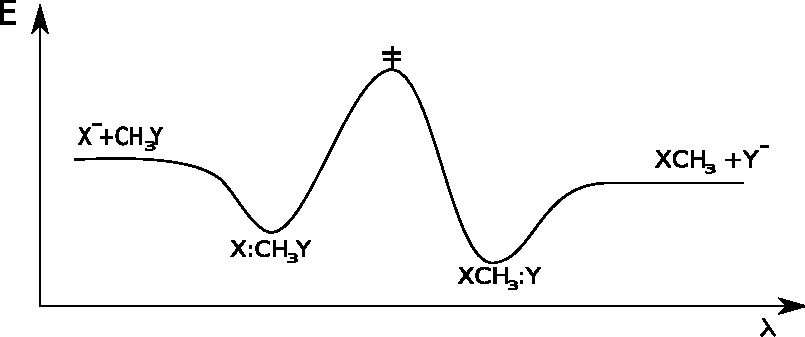
\includegraphics[height=4cm]{image/ELambdaXCH3Y.pdf}
	\caption{\small Andamento dell'energia (E) rispetto alla coordinata di reazione ($\lambda$).}
	\label{fig:ELambda_Rxn_XCH3Y}
\end{figure}
nel quale si nota la formazione dei complessi $X:CH_3Y$ e $Y:CH_3X$.\\
Se la stessa reazione avvenisse in presenza di un solvente noteremmo l'andamento risontrato in Figura \ref{fig:ELambda_Rxn_XCH3Y_Solvente},
\begin{figure}[htbp]
	\centering
		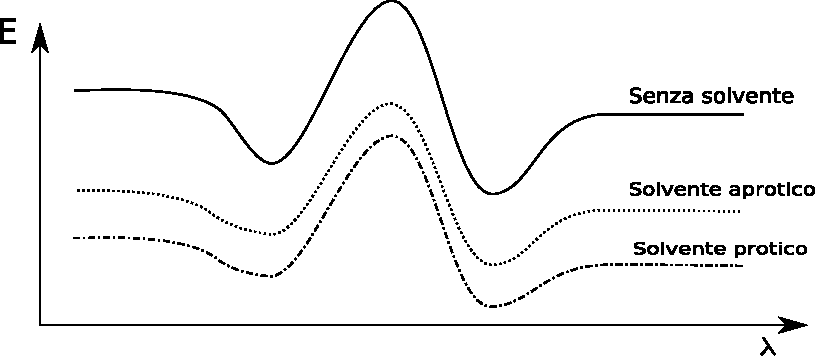
\includegraphics[height=4cm]{image/ELambdaXCH3YSolvente.pdf}
	\caption{\small Andamento dell'energia (E) rispetto alla coordinata di reazione ($\lambda$) per la reazione in soluzione.}
	\label{fig:ELambda_Rxn_XCH3Y_Solvente}
\end{figure}
dove la differenza energetica tra le specie reagenti e quelle in soluzione � definita come $\Delta H$ di solvatazione. Nell'intorno del complesso attivato si ha una diminuzione del $\Delta H_{solv}$ essendo la carica pi� delocalizzata, da cui l'effetto del solvente perde parte della sua importanza, quindi � anche vero che l'energia di attivazione per le reazioni in soluzione � maggiore che non per le specie pure.

Altro fattore importante all'interno delle reazioni in soluzione � il tipo di controllo che la reazione subsce, infatti:
\begin{equation}
	A + B \rightleftharpoons AB \rightleftharpoons AB^{\ddagger} \rightarrow C
	\label{eq:sol:RxnGenerica2}
\end{equation}

Il controllo � di tipo \textsl{cinetico} se la velocit� di formazione del complesso attivato $AB^{\ddagger}$ a determinare la velocit� di reazione.

Il controllo � di tipo \textsl{diffusivo} se la velocit� di formazione del complesso $AB$ a determinare la velocit� di reazione.

Consideriamo il caso di trovarci sotto controllo diffusivo abbiamo:
\begin{equation}
	R = \frac{k_B \cdot T}{h} \cdot [AB^{\ddagger}]
	\label{eq:sol:VelocitaReazione}
\end{equation}
essendo immediata la formazione del complesso attivato la sua reazione sar� all'equilibrio, quindi:
\begin{equation}
	K_{eq}^{\ddagger} = \frac{[AB^{\ddagger}]}{[A] \cdot [B]} = \frac{a_{AB^{\ddagger}}}{a_A \cdot a_B}
	\label{eq:sol:KeqIntermedio}
\end{equation}
essendo anche $a_i = {C_i} \cdot \gamma_i$ ricaviamo:
\begin{equation}
	K_{eq}^{\ddagger} = \frac{C_{AB^{\ddagger}}}{C_A \cdot C_B} \cdot
											\frac{\gamma_{AB^{\ddagger}}}{\gamma_A \cdot \gamma_B}
	\label{eq:sol:KeqIntermedioGamma}
\end{equation}
da cui si ricava:
\begin{equation}
	R = \frac{k_B \cdot T}{h} \cdot K_{eq}^{\ddagger} \cdot
			\frac{\gamma_{AB^{\ddagger}}}{\gamma_A \cdot \gamma_B} \cdot
			C_A \cdot C_B
	\label{eq:sol:ConcIntermedio}
\end{equation}
Essendo anche:
\begin{equation}
	\frac{k_B \cdot T}{h} \cdot K_{eq}^{\ddagger} = cost = K_{(T)}^0
	\label{eq:sol:K0T}
\end{equation}
e riunendo
\begin{equation}
	 K_{(T)} = K_{(T)}^0 \cdot \frac{\gamma_{AB^{\ddagger}}}{\gamma_A \cdot \gamma_B}
	\label{eq:sol:KT}
\end{equation}
otterremmo:
\begin{equation}
	R = K_{(T)} \cdot C_A \cdot C_B
	\label{eq:sol:VelReazioneKo}
\end{equation}

\section{Teoria di Br�nsted-Bjerron}
La determinazione del coefficiente di attivit� delle specie in soluzione pu� essere ottenuta dalle teoria di Br�nsted\footnote{Br�nsted, Johannes, chimico danese.}-Bjerron\footnote{Chi era...} che deriva della teoria di Debye\footnote{Debye, Peter Joseph Wilhelm (Maastricht 1884 - Ithaca, New York 1966), fisico-chimico statunitense di origine olandese.}-H\"uckel\footnote{H\"uckel, Erich assistente di Debye.}.

Queste teorie sono valide per le specie ioniche (in cui � importante l'effetto solvente) e i coefficienti di attivit� si possono ottenere da:
\begin{equation}
	\ln \gamma_i = -0,509 \cdot z_i^2 \cdot \sqrt{I}
	\label{eq:sol:lnGamma}
\end{equation}
dove indichiamo con:
\begin{equation}
	I = \frac{1}{2} \cdot \sum_j m_j z_j^2
	\label{eq:sol:IDebyeHuchel}
\end{equation}
dove $m_j$ indica la molalit� della specie $j$-esima in soluzione e $z_j$ la carica dello ione.

Per quanto visto prima (equazione \ref{eq:sol:KT}), logaritmando, abbiamo:
\begin{equation}
	\log K_{(T)} = \log K_{(T)}^0 + \log \gamma_{AB^{\ddagger}} - \log \gamma_A  - \log \gamma_B
	\label{eq:sol:logKT}
\end{equation}
e per la teoria di Debye-H\"uckel otteniamo:
\begin{equation}
	\frac{\log K_{(T)}}{\log K_{(T)}^0} = - 0,509 \cdot z_{AB^{\ddagger}}^2 \cdot \sqrt{I} +
																					0,509 \cdot z_A^2 \cdot \sqrt{I} +
																					0,509 \cdot z_B^2 \cdot \sqrt{I}
	\label{eq:sol:logKT}
\end{equation}
Per la legge della conservazione delle cariche $z_{AB^{\ddagger}} = z_A + z_B$ e quindi:
\begin{equation}
	\frac{\log K_{(T)}}{\log K_{(T)}^0} = - 0,509 \cdot \sqrt{I} \cdot 
								\left[ z_A^2 + z_B^2 - (z_A + z_B)^2 \right] = 
								-1,018 \cdot \sqrt{I} \cdot z_A \cdot z_B
	\label{eq:sol:logKTFinale}
\end{equation}

% \chapter{Cinetica enzimatica}

	\appendix
		\chapter{Tabella degli integrali}
Data la funzione $f_{(n)}$ definita come:
\begin{equation}
	f_{(n)} = \int_0^{\infty} n^x \cdot e^{-\alpha \cdot x^2} d x
	\label{eq:AppA:IntegraleGenerico}
\end{equation}
con $\alpha > 0$ abbiamo:
\begin{table*}[h]
	\centering
		\begin{tabular}{lr}
			n		&		$f_{(n)}$ \\ \hline
			0		&		$\frac{1}{2} \sqrt{\frac{\pi}{\alpha}} $  			\vspace{0.2cm} \\ \hline
			1		&		$\frac{1}{2 \alpha}$ 														\vspace{0.2cm} \\ \hline
			2		&		$\frac{1}{4} \sqrt{\frac{\pi}{\alpha^3}} $ 			\vspace{0.2cm} \\ \hline
			3		&		$\frac{1}{2 \alpha^2}$ 													\vspace{0.2cm} \\ \hline
			4		&		$\frac{3}{8} \sqrt{\frac{\pi}{\alpha?5}} $ 			\vspace{0.2cm} \\ \hline
			5		&		$\frac{1}{\alpha^3}$ 														\vspace{0.2cm} \\ \hline
			6		&		$\frac{15}{16} \sqrt{\frac{\pi}{\alpha^7}} $ 		\vspace{0.2cm} \\ \hline
			7		&		$\frac{3}{\alpha^4}$ 														\vspace{0.2cm} \\ \hline
		\end{tabular}
\end{table*}

Si noti, anche, che per $n$ pari vale la seguente regola:
\begin{equation}
	\int_{-\infty}^{\infty} n^x \cdot e^{-\alpha \cdot x^2} d x = 2 \cdot f_{(n)}
	\label{eq:AppA:IntegraleGenericoPari}
\end{equation}
mentre per per $n$ dispari:
\begin{equation}
	\int_{-\infty}^{\infty} n^x \cdot e^{-\alpha \cdot x^2} d x = 0
	\label{eq:AppA:IntegraleGenericoDispari}
\end{equation}
		
	\listoffigures
%	\listoftables	
\end{document}